%======================================================================
% chapter07_slides.tex
% Chapter 7: Direct Methods
% Algorithms for Optimization, 2nd Edition (2026)
% Kochenderfer & Wheeler
% Reader-friendly edition: self-contained, complete sentences,
% symbol explanations, worked examples, Greek pronunciations.
%======================================================================
\documentclass[aspectratio=169,10pt]{beamer}

\usetheme{Madrid}
\usecolortheme{seahorse}

\usepackage{amsmath,amssymb,amsfonts}
\usepackage{mathtools}
\usepackage{graphicx}
\usepackage{booktabs}
\usepackage[dvipsnames,svgnames,x11names]{xcolor}
\definecolor{navy}{rgb}{0.0,0.0,0.5}
\usepackage{listings}
\usepackage{algorithm}
\usepackage{algpseudocode}
\usepackage{tikz}
\usetikzlibrary{shapes.geometric, arrows.meta, positioning}
\usepackage{multicol}
\usepackage{array}
\usepackage{colortbl}
\usepackage{enumerate}

\graphicspath{{figures/}}

% ── listings style for Python ──────────────────────────────────────
\lstdefinestyle{python}{
  language=Python,
  basicstyle=\ttfamily\scriptsize,
  keywordstyle=\color{blue!70!black}\bfseries,
  commentstyle=\color{green!50!black}\itshape,
  stringstyle=\color{orange!80!black},
  numbers=left,
  numberstyle=\tiny\color{gray},
  numbersep=5pt,
  frame=single,
  rulecolor=\color{gray!40},
  backgroundcolor=\color{gray!7},
  showstringspaces=false,
  tabsize=4,
  breaklines=true,
  columns=fullflexible,
  keepspaces=true,
}

\setbeamertemplate{footline}[frame number]
\setbeamertemplate{navigation symbols}{}

% ── Title info ─────────────────────────────────────────────────────
\title[Chapter 7: Direct Methods]%
      {\textbf{Chapter 7: Direct Methods}}
\subtitle{Algorithms for Optimization, 2nd Edition (2026)}
\author{Kochenderfer \& Wheeler}
\institute{MIT Press}
\date{}

%======================================================================
\begin{document}
%======================================================================

%──────────────────────────────────────────────────────────────────────
\begin{frame}
  \titlepage
\end{frame}

%──────────────────────────────────────────────────────────────────────
\begin{frame}{Chapter 7 Overview}
  \begin{columns}[T]
    \column{0.55\textwidth}
      \tableofcontents[sectionstyle=show,subsectionstyle=show]
    \column{0.42\textwidth}
      \begin{block}{What are Direct Methods?}
        \textbf{Direct methods} --- also called \emph{zero-order},
        \emph{black-box}, \emph{pattern search}, or
        \emph{derivative-free} methods --- rely \textbf{solely on the
        objective function} $f(\mathbf{x})$ to guide the search.
        They do \emph{not} compute or use the gradient (first
        derivative) or Hessian (second derivative) of $f$.

        \medskip
        This makes them the method of choice whenever derivatives are
        unavailable, unreliable, or expensive to obtain --- for example,
        when $f$ is the output of a simulation, an experiment, or a
        legacy black-box program.  Instead of derivatives, direct
        methods use geometric or heuristic criteria to choose the next
        point to evaluate.
      \end{block}
  \end{columns}
\end{frame}

\AtBeginSection[]{
  \begin{frame}{Outline}
    \tableofcontents[currentsection]
  \end{frame}
}

%======================================================================
\section{Cyclic Coordinate Search}
%======================================================================

\begin{frame}[allowframebreaks]{7.1 Cyclic Coordinate Search --- Concept}
  \textbf{The simplest direct method} is to optimise one variable at a
  time while holding every other variable fixed.  We cycle through each
  coordinate direction in turn, performing a one-dimensional line search
  along that direction, and then repeat until convergence.  Because each
  step is aligned with a coordinate axis, the approach is sometimes
  called \emph{taxicab search} or \emph{coordinate descent}.

  \begin{block}{Definition: Cyclic Coordinate Search}
    Given an objective function $f : \mathbb{R}^n \to \mathbb{R}$
    (where $n$ is the number of variables) and a current point
    $\mathbf{x}^{(k)}$ (read: ``$\mathbf{x}$ at iteration $k$''),
    the method updates each coordinate one at a time:
    \begin{align}
      x_2^{(1)} &= \underset{x_2}{\arg\min}\;
                   f\!\bigl(x_1^{(1)},\,x_2,\,x_3^{(1)},\ldots,x_n^{(1)}\bigr)
                   \tag{7.1} \\[4pt]
      x_3^{(2)} &= \underset{x_3}{\arg\min}\;
                   f\!\bigl(x_1^{(1)},\,x_2^{(1)},\,x_3,\ldots,x_n^{(1)}\bigr)
                   \tag{7.2}
    \end{align}
  \end{block}

  \begin{block}{Notation}
    In equation (7.1): $x_2^{(1)}$ (``$x$-sub-2 superscript 1'')
    means the updated value of the second variable after the first
    line search.  The notation $\arg\min_{x_2}$ (``argmin over $x_2$'')
    means ``the value of $x_2$ that minimises''.  All other variables
    $x_1^{(1)}, x_3^{(1)}, \ldots, x_n^{(1)}$ are held fixed at
    their current values.  The superscript $(1)$ on $x_j^{(1)}$ means
    the value of variable $j$ after the first full cycle.
  \end{block}

  Each step is along one of the $n$ \textbf{basis vectors}
  (also called coordinate directions or standard unit vectors):
  \[
    \mathbf{e}^{(i)} \in \mathbb{R}^n, \qquad
    e^{(i)}_k = \begin{cases}1 & k = i \\ 0 & \text{otherwise}\end{cases}
  \]

  \begin{block}{Notation: Basis Vector}
    $\mathbf{e}^{(i)}$ (``$e$ superscript $i$'') is a vector of
    length $n$ that is all zeros except for a $1$ in position $i$.
    For example, in two dimensions: $\mathbf{e}^{(1)} = [1,\,0]^\top$
    and $\mathbf{e}^{(2)} = [0,\,1]^\top$.  Line-searching along
    $\mathbf{e}^{(i)}$ means moving only in the $i$-th variable.
  \end{block}

  \begin{columns}[T]
    \column{0.54\textwidth}
      \begin{exampleblock}{Worked Example (2D)}
        Let $f(x_1, x_2) = x_1^2 + 2x_2^2$, starting at
        $\mathbf{x} = [3,\,2]^\top$.

        \textbf{Step 1 --- optimise over $x_1$, holding $x_2 = 2$:}
        We minimise $g_1(x_1) = x_1^2 + 2(2)^2 = x_1^2 + 8$.
        The minimum is at $x_1 = 0$, so we move to $[0,\,2]^\top$.

        \textbf{Step 2 --- optimise over $x_2$, holding $x_1 = 0$:}
        We minimise $g_2(x_2) = 0 + 2x_2^2$.
        The minimum is at $x_2 = 0$, so we arrive at $[0,\,0]^\top$.

        In this example the algorithm converged in one cycle because the
        function is separable (each variable appears independently).
        For a function like Rosenbrock where the variables are coupled,
        many more cycles are needed.
      \end{exampleblock}
    \column{0.43\textwidth}
      \begin{center}
        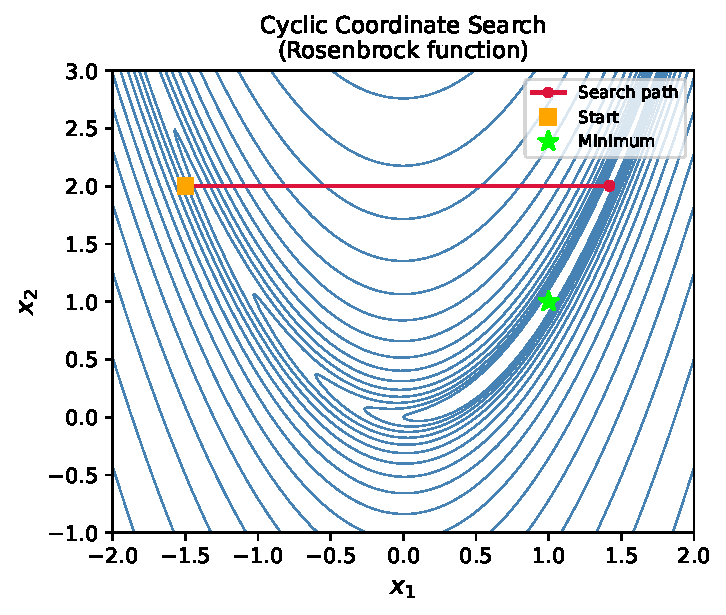
\includegraphics[width=\linewidth]{fig_cyclic_coordinate.pdf}\\
        {\scriptsize Cyclic coordinate search applied to the Rosenbrock
        function.  The path alternates between the two coordinate
        directions, zigzagging toward the minimum at $(1,\,1)$.}
      \end{center}
  \end{columns}

  \begin{alertblock}{Key Insight}
    Cyclic coordinate search is easy to implement and works well when
    the objective function is \emph{separable} --- meaning each variable
    contributes independently to $f$.  However, when the level curves
    of $f$ are tilted diagonally, the method must take many small steps
    to move diagonally, because each individual step is locked to a
    coordinate axis.  This is the fundamental weakness of the method.
  \end{alertblock}
\end{frame}

\begin{frame}[allowframebreaks]{7.1 Cyclic Coordinate Search --- Algorithm and Acceleration}
  \begin{columns}[T]
    \column{0.52\textwidth}
      \begin{alertblock}{Algorithm 7.1 --- Cyclic Coordinate Search}
        \textbf{Inputs:} the function $f$, starting point
        $\mathbf{x}^{(1)}$, and a stopping tolerance $\epsilon$
        (epsilon, pronounced ``eps-ill-on'') --- the minimum movement
        in $\mathbf{x}$ considered significant.

        \begin{enumerate}\setlength\itemsep{2pt}
          \item Set $\Delta = \infty$ (Delta, the change in position),
                $n = \text{length}(\mathbf{x})$
          \item \textbf{while} $\Delta > \epsilon$:
          \item \quad Save current position: $\mathbf{x}' \leftarrow \mathbf{x}$
          \item \quad \textbf{for} $i = 1,\ldots,n$:
          \item \qquad Set direction $d \leftarrow \mathbf{e}^{(i)}$
          \item \qquad Update: $\mathbf{x} \leftarrow \texttt{line\_search}(f,\mathbf{x},d)$
          \item \quad Measure movement: $\Delta \leftarrow \|\mathbf{x} - \mathbf{x}'\|$
          \item \textbf{return} $\mathbf{x}$
        \end{enumerate}
      \end{alertblock}

      \begin{block}{Reading the Algorithm}
        The loop keeps cycling through all $n$ coordinate directions,
        each time doing a one-dimensional line search to find the best
        step along that direction.  After one full pass through all $n$
        directions, the algorithm checks how far the current point
        $\mathbf{x}$ has moved from the start of the cycle $\mathbf{x}'$.
        The notation $\|\mathbf{x} - \mathbf{x}'\|$ (the Euclidean
        distance between the two points) measures the total displacement.
        If this distance is smaller than $\epsilon$ (epsilon), the
        algorithm concludes it is no longer making meaningful progress
        and stops.
      \end{block}
    \column{0.45\textwidth}
      \begin{block}{Acceleration Step}
        After a full cycle that moves from $\mathbf{x}'$ to $\mathbf{x}$,
        we can add one more line search along the direction of net
        movement:
        \[
          \mathbf{x}^{(k+1)} \leftarrow
          \texttt{line\_search}\!\left(f,\;\mathbf{x},\;\mathbf{x}-\mathbf{x}'\right)
        \]
        The idea is that if the algorithm consistently moved in a
        direction over a whole cycle, then taking an additional step
        in that same direction is likely to be beneficial.  This
        ``momentum'' step can significantly reduce the number of
        cycles required to converge on diagonal valleys.
      \end{block}

      \begin{center}
        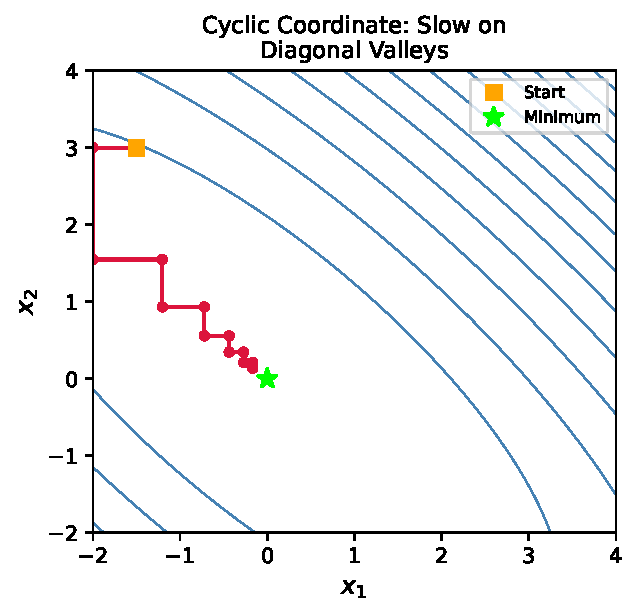
\includegraphics[width=\linewidth]{fig_cyclic_stuck.pdf}\\
        {\scriptsize Cyclic search on a diagonally-oriented valley.
        The method gets stuck taking tiny zigzag steps along the
        axis directions instead of moving directly down the valley.}
      \end{center}
  \end{columns}
\end{frame}

\begin{frame}[fragile]{7.1 Cyclic Coordinate Search --- Python Implementation}
\begin{lstlisting}[style=python, caption={Cyclic coordinate search in Python (NumPy/SciPy)}]
import numpy as np
from scipy.optimize import minimize_scalar

def cyclic_coordinate_search(f, x0, eps=1e-6, max_cycles=200):
    """
    Cyclic coordinate search (coordinate descent with line search).
    f  : objective function R^n -> R
    x0 : initial point (array-like)
    eps: stopping tolerance on the change in x per cycle
    """
    x = np.array(x0, dtype=float)
    n = len(x)
    for _ in range(max_cycles):
        x_prev = x.copy()
        for i in range(n):
            # Line search along the i-th coordinate direction.
            # We fix all other coordinates and minimise over x[i].
            def fi(t):
                xc = x.copy()
                xc[i] = t
                return f(xc)
            result = minimize_scalar(fi, bracket=(x[i]-2, x[i]+2),
                                     method='brent')
            x[i] = result.x
        if np.linalg.norm(x - x_prev) < eps:
            break
    return x

# Example: Rosenbrock function  f(x1, x2) = (1-x1)^2 + 100*(x2-x1^2)^2
# Minimum is at (1, 1).
f = lambda v: (1 - v[0])**2 + 100*(v[1] - v[0]**2)**2
x_opt = cyclic_coordinate_search(f, x0=[-1.2, 1.0])
print(f"Optimum: {x_opt}")   # -> approx [1.0, 1.0]
\end{lstlisting}
\end{frame}

%======================================================================
\section{Powell's Method}
%======================================================================

\begin{frame}[allowframebreaks]{7.2 Powell's Method --- Motivation and Conjugate Directions}
  \textbf{Cyclic coordinate search gets stuck on diagonal valleys}
  because it can only move along axis-aligned directions.
  Powell's method (Michael J. D. Powell, 1964) fixes this by
  gradually building up a set of \emph{conjugate} search directions
  that are better adapted to the shape of the objective function.
  Unlike the fixed coordinate directions, these new directions
  can point diagonally, allowing the algorithm to follow curved
  valleys directly.

  \begin{columns}[T]
    \column{0.54\textwidth}
      \begin{block}{Definition: Conjugate Directions}
        Two directions $\mathbf{u}$ and $\mathbf{v}$ are called
        \textbf{conjugate} with respect to a matrix
        $\mathbf{Q}$ (the Hessian of $f$) if:
        \[
          \mathbf{u}^\top \mathbf{Q}\, \mathbf{v} = 0
        \]
        This is a generalisation of orthogonality.
      \end{block}

      \begin{block}{Notation}
        Here $\mathbf{u}^\top$ (``$\mathbf{u}$ transpose'') denotes
        the row vector version of $\mathbf{u}$, so
        $\mathbf{u}^\top \mathbf{Q}\, \mathbf{v}$ is a scalar
        (a single number) obtained by multiplying a row vector, a
        matrix, and a column vector together.  The matrix
        $\mathbf{Q}$ encodes how the function curves in different
        directions --- it is the matrix of second partial derivatives.
        Two directions are conjugate when this scalar product equals zero.
      \end{block}

      \begin{alertblock}{Why Conjugacy Matters}
        For a quadratic objective
        $f(\mathbf{x}) = \tfrac{1}{2}\mathbf{x}^\top\mathbf{Q}\mathbf{x}
        + \mathbf{b}^\top\mathbf{x}$
        (which approximates any smooth function near its minimum),
        line-searching along $n$ mutually conjugate directions finds
        the global minimum in \emph{exactly} $n$ steps, regardless of
        the problem's conditioning.  This gives Powell's method
        superlinear convergence near the minimum.
      \end{alertblock}
    \column{0.43\textwidth}
      \begin{center}
        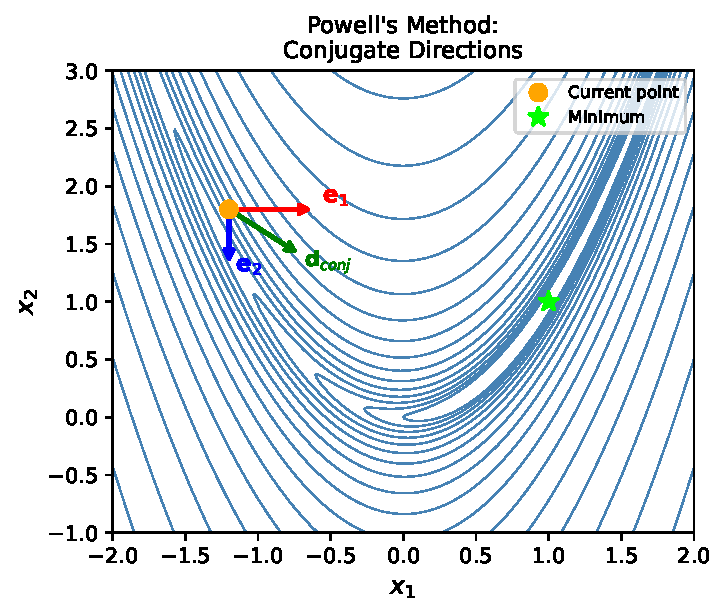
\includegraphics[width=0.9\linewidth]{fig_powell.pdf}\\
        {\scriptsize Powell's method on a quadratic function.  Starting
        from coordinate directions, the algorithm quickly builds up
        diagonal conjugate directions that point along the valley and
        reaches the minimum in far fewer steps than cyclic search.}
      \end{center}

      \begin{block}{Key Idea: How New Directions Are Built}
        After each full cycle of $n$ line searches, the \emph{net
        displacement} of the point,
        $\mathbf{d}^{(\text{new})} = \mathbf{x}^{(k+1)} - \mathbf{x}^{(k)}$,
        automatically tends to be conjugate to all the previous
        search directions.  Powell's method uses this net displacement
        as the new search direction for the next cycle, dropping the
        oldest direction to maintain a set of $n$ directions.
      \end{block}
  \end{columns}
\end{frame}

\begin{frame}[allowframebreaks]{7.2 Powell's Method --- Algorithm}
  \begin{columns}[T]
    \column{0.52\textwidth}
      \begin{alertblock}{Algorithm 7.4 --- Powell's Method}
        \textbf{Inputs:} function $f$, starting point $\mathbf{x}$,
        tolerance $\epsilon$ (epsilon).

        \begin{enumerate}\setlength\itemsep{1pt}
          \item Initialise $U \leftarrow [\mathbf{e}^{(1)},\ldots,\mathbf{e}^{(n)}]$
                (the $n$ coordinate basis directions as column vectors)
          \item Set $\Delta \leftarrow \infty$
          \item \textbf{while} $\Delta > \epsilon$:
          \item \quad Save: $\mathbf{x}' \leftarrow \mathbf{x}$
          \item \quad \textbf{for} $i = 1,\ldots,n$: \hfill
                (line search along each direction)
          \item \qquad $d \leftarrow U[i]$
          \item \qquad $\mathbf{x} \leftarrow \texttt{line\_search}(f,\mathbf{x},d)$
          \item \quad \textbf{for} $i = 1,\ldots,n-1$: \hfill
                (shift directions: drop oldest)
          \item \qquad $U[i] \leftarrow U[i+1]$
          \item \quad $U[n] \leftarrow \mathbf{x} - \mathbf{x}'$
                \hfill (add net displacement as new direction)
          \item \quad $\mathbf{x} \leftarrow
                \texttt{line\_search}(f,\mathbf{x}',U[n])$
                \hfill (search along new direction from start of cycle)
          \item \quad $\Delta \leftarrow \|\mathbf{x} - \mathbf{x}'\|$
          \item \textbf{return} $\mathbf{x}$
        \end{enumerate}
      \end{alertblock}
    \column{0.45\textwidth}
      \begin{block}{Reading the Algorithm Step by Step}
        \textbf{Step 1} initialises the search directions to the
        standard coordinate axes --- just like cyclic search.

        \textbf{Steps 4--7} perform one full cycle of $n$ line searches,
        one along each current direction, advancing $\mathbf{x}$ each
        time.

        \textbf{Steps 8--11} update the direction set.  The oldest
        direction $U[1]$ is discarded and every direction shifts one
        position.  The \emph{net displacement} from the start to the
        end of the cycle, $\mathbf{x} - \mathbf{x}'$, becomes the new
        last direction $U[n]$.  A final line search is then performed
        along this new direction starting from $\mathbf{x}'$.

        \textbf{Step 12} measures convergence as the Euclidean distance
        moved during the cycle.
      \end{block}

      \begin{block}{Convergence Guarantee}
        For a quadratic objective in $n$ variables, Powell's method
        converges in exactly $n$ cycles.  For non-quadratic functions
        it converges super-linearly near the minimum.  The method
        automatically adapts step sizes through the line searches ---
        it does not need a learning rate to be set manually.
      \end{block}
  \end{columns}
\end{frame}

\begin{frame}[fragile]{7.2 Powell's Method --- Python Implementation}
\begin{lstlisting}[style=python, caption={Powell's method (Python/SciPy)}]
import numpy as np
from scipy.optimize import minimize_scalar, minimize

def powell(f, x0, eps=1e-8, max_iter=200):
    """
    Powell's method for unconstrained minimisation.
    f  : callable  R^n -> R
    x0 : initial point (1-D array)
    eps: stopping tolerance
    """
    x = np.array(x0, dtype=float)
    n = len(x)
    U = np.eye(n)   # start with n coordinate directions

    for _ in range(max_iter):
        x_prev = x.copy()
        # Cycle through all current search directions
        for i in range(n):
            d = U[i]
            res = minimize_scalar(lambda t: f(x + t * d))
            x = x + res.x * d
        # Shift directions: drop oldest, add net displacement
        U[:-1] = U[1:]
        U[-1] = x - x_prev
        norm = np.linalg.norm(U[-1])
        if norm > 1e-12:
            d = U[-1]
            # Line search along the new direction from start of cycle
            res = minimize_scalar(lambda t: f(x_prev + t * d))
            x = x_prev + res.x * d
        if np.linalg.norm(x - x_prev) < eps:
            break
    return x

# SciPy has a built-in, highly optimised Powell implementation:
result = minimize(lambda v: (1-v[0])**2 + 100*(v[1]-v[0]**2)**2,
                  [-1.2, 1.0], method='Powell')
print(result.x)   # -> [1.0, 1.0]
\end{lstlisting}
\end{frame}

%======================================================================
\section{Hooke-Jeeves Method}
%======================================================================

\begin{frame}[allowframebreaks]{7.3 Hooke-Jeeves Method --- Concept}
  The \textbf{Hooke-Jeeves method} (Robert Hooke and T.~A. Jeeves,
  1961) is a derivative-free method that uses small exploratory steps
  to probe the neighbourhood of the current point, and then capitalises
  on any improvement by taking a larger \emph{pattern move} in the
  same direction.  The intuition is simple: if taking a small step in
  some direction improved the objective, then it is likely worthwhile
  to continue moving in that direction.

  \begin{columns}[T]
    \column{0.54\textwidth}
      \begin{block}{Two-Phase Iteration}
        Each iteration of the Hooke-Jeeves method has two phases:

        \textbf{Phase 1 --- Exploratory Search.}
        Starting from the current \emph{anchor point}
        $\mathbf{x}^{(\text{base})}$, probe the neighbourhood by
        trying a small step $\pm\alpha\,\mathbf{e}^{(i)}$ (``plus or
        minus alpha times e-superscript-i'') in each coordinate
        direction $i$, where $\alpha$ (alpha) is the current step size.
        Accept whichever probe improves $f$ most.  If neither
        $+\alpha\,\mathbf{e}^{(i)}$ nor $-\alpha\,\mathbf{e}^{(i)}$
        improves $f$, keep the current point for dimension $i$.

        \textbf{Phase 2 --- Pattern Move.}
        If the exploratory search found an improvement, take an extra
        step in the direction of overall improvement:
        \[
          \mathbf{x}^{(\text{pattern})} =
          \mathbf{x}^{(k+1)} + \bigl(\mathbf{x}^{(k+1)} - \mathbf{x}^{(k)}\bigr)
        \]
        This doubles the step just taken, effectively extrapolating
        along the successful direction.

        If no improvement is found anywhere, reduce the step size:
        $\alpha \leftarrow \alpha / 2$ (halve alpha) and try again.
        The algorithm stops when $\alpha < \epsilon$ (epsilon).
      \end{block}

      \begin{block}{Notation: Pattern Move}
        In the pattern move formula: $\mathbf{x}^{(k+1)}$ is the
        improved point found by the exploratory search, and
        $\mathbf{x}^{(k)}$ is the anchor at the start of the iteration.
        The difference $\mathbf{x}^{(k+1)} - \mathbf{x}^{(k)}$ is
        the displacement vector pointing from the old anchor to the new
        one.  Adding this displacement again to $\mathbf{x}^{(k+1)}$
        gives a point that is one more step further along the same
        direction --- a ``momentum'' move.
      \end{block}

      \begin{alertblock}{Cost per Iteration}
        In the worst case, the exploratory search evaluates
        $f$ at $2n$ points (two probes per dimension: one in the
        positive direction and one in the negative direction).  For
        large $n$ this can be expensive.  In practice, each dimension
        typically needs only one probe, since we move on as soon as we
        find an improvement.
      \end{alertblock}

    \column{0.43\textwidth}
      \begin{center}
        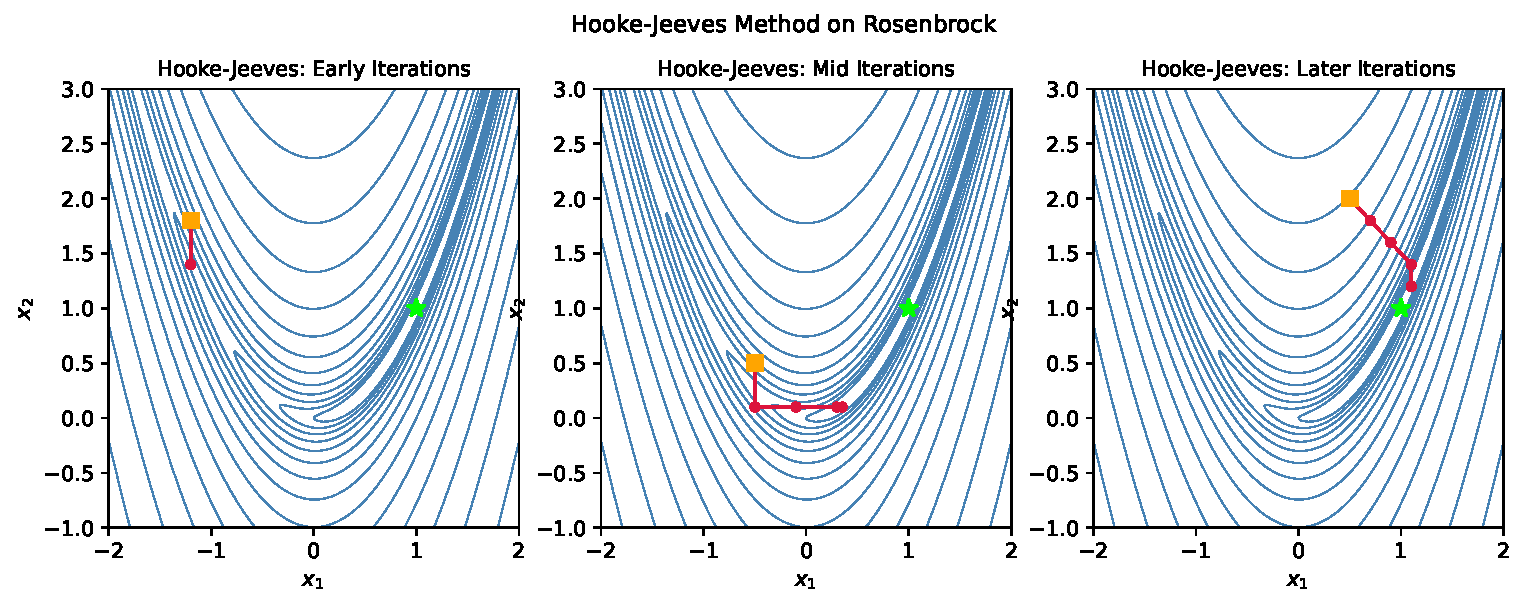
\includegraphics[width=\linewidth]{fig_hooke_jeeves.pdf}\\
        {\scriptsize Hooke-Jeeves applied to the Rosenbrock function.
        Large exploratory steps early on are followed by a step-size
        reduction when the algorithm approaches the curved valley.}
      \end{center}
  \end{columns}
\end{frame}

\begin{frame}[allowframebreaks]{7.3 Hooke-Jeeves Method --- Algorithm and Worked Example}
  \begin{columns}[T]
    \column{0.55\textwidth}
      \begin{alertblock}{Algorithm 7.5 --- Hooke-Jeeves}
        \textbf{Inputs:} $f$, starting point $\mathbf{x}$,
        initial step size $\alpha$ (alpha), tolerance $\epsilon$ (epsilon).
        \begin{enumerate}\setlength\itemsep{1pt}
          \item \textbf{while} $\alpha > \epsilon$:
          \item \quad Save anchor: $\mathbf{x}^{(\text{base})} \leftarrow \mathbf{x}$
          \item \quad \textbf{for} $i = 1,\ldots,n$: \hfill (exploratory)
          \item \qquad Evaluate $f(\mathbf{x} + \alpha\mathbf{e}^{(i)})$
                and $f(\mathbf{x} - \alpha\mathbf{e}^{(i)})$
          \item \qquad Keep whichever reduces $f$; else keep $\mathbf{x}$
          \item \quad \textbf{if} improvement found (i.e., $\mathbf{x} \ne \mathbf{x}^{(\text{base})}$):
          \item \qquad Pattern step:
                $\mathbf{x} \mathrel{+}= \mathbf{x} - \mathbf{x}^{(\text{base})}$
          \item \quad \textbf{else}: \hfill (no improvement found)
          \item \qquad $\alpha \leftarrow \alpha / 2$ \hfill (reduce step size)
          \item \textbf{return} $\mathbf{x}$
        \end{enumerate}
      \end{alertblock}
    \column{0.42\textwidth}
      \begin{exampleblock}{Worked Example (2D)}
        Let $f(x_1,x_2) = x_1^2 + 2x_2^2$, start at
        $\mathbf{x}=[2,\,1]^\top$, initial step $\alpha = 0.5$.

        \textbf{Exploratory phase:}
        \begin{itemize}\setlength\itemsep{1pt}
          \item Try $[2.5,\,1]$: $f = 6.25 + 2 = 8.25$ (worse)
          \item Try $[1.5,\,1]$: $f = 2.25 + 2 = 4.25$ (better \checkmark)
          \item Try $[1.5,\,1.5]$: $f = 2.25 + 4.5 = 6.75$ (worse)
          \item Try $[1.5,\,0.5]$: $f = 2.25 + 0.5 = 2.75$ (better \checkmark)
        \end{itemize}
        After exploration: $\mathbf{x} = [1.5,\,0.5]^\top$.

        \textbf{Pattern move:}
        Displacement $= [1.5,0.5] - [2,1] = [-0.5,\,-0.5]$.
        New point: $[1.5,0.5] + [-0.5,-0.5] = [1.0,\,0.0]^\top$.
        Check: $f([1.0,\,0.0]) = 1.0$ (better than $2.75$).

        The pattern move jumped the point closer to the minimum
        at $[0,\,0]$ in one step.
      \end{exampleblock}
  \end{columns}

  \begin{block}{Convergence Properties}
    The Hooke-Jeeves method is provably convergent for continuous
    functions: as the step size $\alpha$ shrinks to zero, the
    sequence of iterates must accumulate at a stationary point.
    However, like all local methods it can converge to a local minimum
    rather than the global minimum.  The rate of convergence is
    linear (i.e., the error reduces by a constant factor each iteration),
    which is slower than methods that use derivative information.
  \end{block}
\end{frame}

\begin{frame}[fragile]{7.3 Hooke-Jeeves --- Python Implementation}
\begin{lstlisting}[style=python, caption={Hooke-Jeeves method in Python}]
import numpy as np

def hooke_jeeves(f, x0, alpha=1.0, eps=1e-6):
    """
    Hooke-Jeeves (pattern search) method.
    f     : callable R^n -> R
    x0    : initial point
    alpha : initial step size (alpha, controls exploration radius)
    eps   : stopping tolerance (stop when alpha < eps)
    """
    x = np.array(x0, dtype=float)
    n = len(x)
    while alpha > eps:
        x_base  = x.copy()      # save the anchor point
        x_trial = x.copy()      # start exploration from here
        improved = False
        for i in range(n):
            for sign in (1, -1):
                x_new = x_trial.copy()
                x_new[i] += sign * alpha
                if f(x_new) < f(x_trial):
                    x_trial = x_new
                    improved = True
                    break          # accept first improvement
        if improved:
            # Pattern move: step in same direction as net displacement
            x = x_trial + (x_trial - x_base)
        else:
            alpha *= 0.5           # reduce step size by half

    return x

# Demo: minimum of f at (0, 0)
f = lambda v: v[0]**2 + 2*v[1]**2
x_opt = hooke_jeeves(f, x0=[2.0, 1.0])
print(f"Optimum: {x_opt}")   # -> [~0, ~0]
\end{lstlisting}
\end{frame}

%======================================================================
\section{Generalized Pattern Search}
%======================================================================

\begin{frame}[allowframebreaks]{7.4 Generalized Pattern Search --- Overview}
  The Hooke-Jeeves method uses the $\pm\mathbf{e}^{(i)}$ coordinate
  directions for its exploratory steps.  \textbf{Generalized Pattern
  Search} (GPS) relaxes this restriction and allows \emph{any} set of
  directions $\mathcal{D}$, provided that set satisfies a key
  geometric condition: it must be a \emph{positive spanning set}.
  This generalisation allows the search to explore diagonal directions
  from the start, and also enables the method to handle constrained
  problems where some coordinate directions would leave the feasible
  region.

  \begin{columns}[T]
    \column{0.54\textwidth}
      \begin{block}{Definition: Positive Spanning Set}
        A set of vectors
        $\mathcal{D} = \{\mathbf{d}^{(1)},\ldots,\mathbf{d}^{(m)}\}$
        is a \textbf{positive spanning set} for $\mathbb{R}^n$ if
        every vector in $\mathbb{R}^n$ can be written as a
        \textbf{non-negative} linear combination of vectors in
        $\mathcal{D}$.  Formally:
        \[
          \forall\;\mathbf{v} \in \mathbb{R}^n,\;
          \exists\; \lambda^{(i)} \ge 0:\;
          \mathbf{v} = \sum_{i=1}^m \lambda^{(i)} \mathbf{d}^{(i)}
        \]
        At least $m \ge n+1$ directions are required.
      \end{block}

      \begin{block}{Notation}
        The symbol $\forall$ (``for all'') means ``for every choice of
        $\mathbf{v}$''.  The symbol $\exists$ (``there exists'') means
        ``we can find''.  The scalars $\lambda^{(i)}$ (lambda,
        pronounced ``lam-da'') are the non-negative coefficients, each
        $\geq 0$.  The condition $\mathbf{v} = \sum_{i=1}^m \lambda^{(i)}
        \mathbf{d}^{(i)}$ (Sigma, meaning ``sum from $i=1$ to $m$'')
        says that we can decompose any direction $\mathbf{v}$ as a
        sum of the directions in $\mathcal{D}$, with non-negative weights.
      \end{block}

      \begin{alertblock}{How to Read the Positive-Span Condition}
        Intuitively, a positive spanning set ``covers all directions''
        in the sense that for any descent direction (a direction that
        decreases $f$), at least one vector in $\mathcal{D}$ must have
        a positive component along it.  This guarantees that the
        algorithm will find a decreasing direction whenever one exists
        near the current point.  Without this condition, there could
        be a direction of descent that the algorithm never tries.
      \end{alertblock}
    \column{0.43\textwidth}
      \begin{center}
        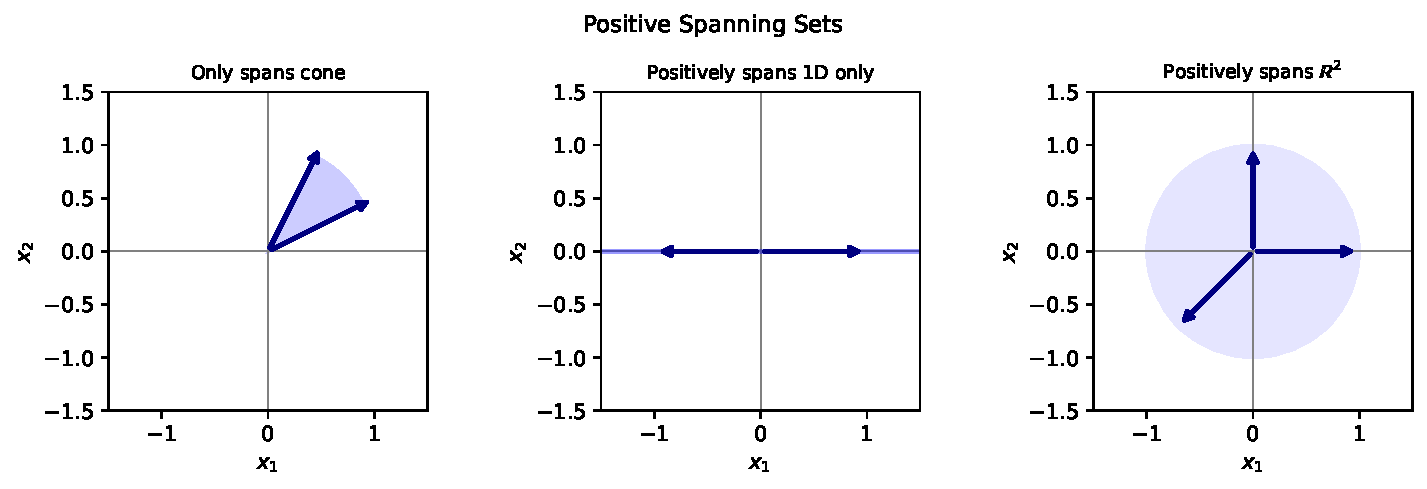
\includegraphics[width=\linewidth]{fig_positive_spanning.pdf}\\
        {\scriptsize Three sets of directions in $\mathbb{R}^2$.
        Left: only spans a cone (not all of $\mathbb{R}^2$).
        Centre: only spans one dimension.
        Right: positively spans all of $\mathbb{R}^2$ --- any
        direction can be expressed as a non-negative combination
        of the shown vectors.}
      \end{center}
      \begin{block}{Minimum Direction Sets for $\mathbb{R}^n$}
        The simplest positive spanning set for $\mathbb{R}^n$ uses
        $2n$ directions: the positive and negative coordinate axes
        $\{+\mathbf{e}^{(i)}, -\mathbf{e}^{(i)}\}$ for $i=1,\ldots,n$.
        But we can also use just $n+1$ directions if they are chosen
        carefully.  Fewer directions means cheaper iterations but
        potentially less exploration.
      \end{block}
  \end{columns}
\end{frame}

\begin{frame}[allowframebreaks]{7.4 Generalized Pattern Search --- Algorithm and Mesh}
  \begin{columns}[T]
    \column{0.52\textwidth}
      \begin{alertblock}{Algorithm 7.6 --- Generalized Pattern Search}
        \textbf{Inputs:} $f$, starting point $\mathbf{x}$, initial step
        $\alpha$ (alpha), direction set $\mathcal{D}$, tolerance $\epsilon$.
        \begin{enumerate}\setlength\itemsep{1pt}
          \item \textbf{while} $\alpha > \epsilon$:
          \item \quad \textbf{for} each direction $\mathbf{d} \in \mathcal{D}$:
          \item \qquad \textbf{if} $f(\mathbf{x} + \alpha\mathbf{d}) < f(\mathbf{x})$:
          \item \qquad\quad Accept: $\mathbf{x} \leftarrow
                \mathbf{x} + \alpha\mathbf{d}$; \textbf{break} (stop iterating $\mathcal{D}$)
          \item \quad \textbf{if} no direction gave improvement:
          \item \qquad Reduce: $\alpha \leftarrow \alpha / 2$
          \item \textbf{return} $\mathbf{x}$
        \end{enumerate}
      \end{alertblock}

      \begin{block}{Reading the Algorithm}
        At each step, the algorithm tries moving in every direction in
        $\mathcal{D}$ (scaled by the current step size $\alpha$) and
        accepts the \emph{first} direction that improves $f$.  If none
        improves $f$, the step size is halved and the process repeats.
        When $\alpha$ falls below the tolerance $\epsilon$, the
        algorithm declares convergence.  Compared to Hooke-Jeeves,
        GPS is identical in spirit but works with any valid direction
        set $\mathcal{D}$.
      \end{block}
    \column{0.45\textwidth}
      \begin{block}{The Mesh Structure}
        A key theoretical property of GPS is that all evaluated points
        lie on a scaled \emph{lattice} (a regularly-spaced grid):
        \[
          \mathbf{x}^{(k)} = \mathbf{x}^{(1)} +
          \alpha^{(k)}\, \mathbf{D}\,\mathbf{z},\quad
          \mathbf{z} \in \mathbb{Z}^m_{\ge 0}
        \]
        where $\mathbf{D}$ is the matrix whose columns are the
        direction vectors, and $\mathbf{z}$ (z) is a vector of
        non-negative integers recording how many steps have been taken
        in each direction.  The lattice is scaled by $\alpha^{(k)}$
        (alpha at iteration $k$) and need not be axis-aligned.
      \end{block}

      \begin{center}
        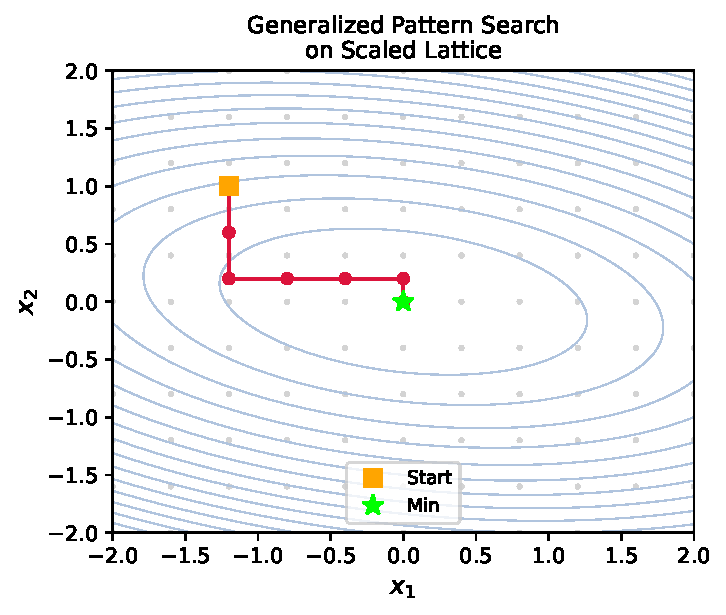
\includegraphics[width=\linewidth]{fig_pattern_search.pdf}\\
        {\scriptsize All previously evaluated points in GPS lie on a
        scaled lattice.  The mesh is not stored explicitly but arises
        automatically from the algorithm's structure.}
      \end{center}

      \begin{block}{Convergence Guarantee}
        Under mild continuity assumptions on $f$, GPS is guaranteed to
        converge to a stationary point.  This is stronger than
        Hooke-Jeeves, which has no such guarantee in the general
        non-smooth case.  The positive-spanning condition is the
        geometric key: it ensures that a descent direction will always
        be found if one exists within the current mesh.
      \end{block}
  \end{columns}
\end{frame}

\begin{frame}[fragile]{7.4 Generalized Pattern Search --- Python Implementation}
\begin{lstlisting}[style=python, caption={Generalized pattern search in Python}]
import numpy as np

def generalized_pattern_search(f, x0, alpha=1.0, eps=1e-6,
                                directions=None):
    """
    Generalized Pattern Search with a user-supplied positive spanning set.
    f          : callable R^n -> R
    x0         : initial point
    alpha      : initial step size
    eps        : stopping tolerance
    directions : array of shape (m, n); defaults to +-e_i (2n directions)
    """
    x = np.array(x0, dtype=float)
    n = len(x)
    if directions is None:
        # Default: coordinate directions + their negatives (2n vectors)
        # This is a positive spanning set for R^n
        directions = np.vstack([np.eye(n), -np.eye(n)])

    while alpha > eps:
        improved = False
        for d in directions:
            x_trial = x + alpha * d
            if f(x_trial) < f(x):
                x = x_trial
                improved = True
                break          # accept first improvement, restart direction loop
        if not improved:
            alpha *= 0.5       # halve step size and retry
    return x

# Example: use a richer positive spanning set for R^2 (6 directions)
# The set {e1, -e1, e2, -e2, e1+e2, -e1-e2} positively spans R^2
custom_dirs = np.array([[1, 0], [-1, 0], [0, 1], [0, -1],
                         [1, 1], [-1, -1]], dtype=float)
f = lambda v: (v[0]-1)**2 + 2*(v[1]+1)**2    # minimum at (1, -1)
x_opt = generalized_pattern_search(f, [0.0, 0.0],
                                    directions=custom_dirs)
print(f"Optimum: {x_opt}")  # -> [~1.0, ~-1.0]
\end{lstlisting}
\end{frame}

%======================================================================
\section{Nelder-Mead Simplex Method}
%======================================================================

\begin{frame}[allowframebreaks]{7.5 Nelder-Mead --- Simplex Concept and Setup}
  The \textbf{Nelder-Mead simplex method} (John Nelder and Roger
  Mead, 1965) maintains a geometric shape called a \emph{simplex}
  and repeatedly deforms it to move toward and shrink around the
  minimum.  Rather than searching along fixed directions, the simplex
  is a living shape that adapts to the landscape of $f$.  It is
  arguably the most widely used derivative-free method in practice,
  and is the default method in SciPy's \texttt{minimize} function when
  no gradient is provided.

  \begin{columns}[T]
    \column{0.54\textwidth}
      \begin{block}{What is a Simplex?}
        A \textbf{simplex} in $\mathbb{R}^n$ is the simplest possible
        $n$-dimensional shape: it has exactly $n+1$ vertices.
        \begin{itemize}\setlength\itemsep{2pt}
          \item In $n=1$ dimension: a line segment (2 endpoints)
          \item In $n=2$ dimensions: a triangle (3 vertices)
          \item In $n=3$ dimensions: a tetrahedron (4 vertices)
        \end{itemize}
        The idea is to evaluate $f$ at all $n+1$ vertices and then
        move the \emph{worst} vertex (the one with the highest function
        value) to a better location using geometric operations.
      \end{block}

      \begin{block}{Notation: Sorting the Vertices}
        Sort the $n+1$ vertices of the simplex by their function values:
        \[
          y_l \le y_{s} \le \cdots \le y_h
        \]
        where the subscripts stand for:
        \begin{itemize}\setlength\itemsep{1pt}
          \item $y_l$ and $\mathbf{x}_l$: the \textbf{lowest} (best)
                value and its vertex --- this is the current best point.
          \item $y_s$ and $\mathbf{x}_s$: the \textbf{second-highest}
                value --- used as a threshold for deciding operations.
          \item $y_h$ and $\mathbf{x}_h$: the \textbf{highest} (worst)
                value and its vertex --- this is the vertex we move.
          \item $\bar{\mathbf{x}}$ (``$\mathbf{x}$-bar''): the
                \textbf{centroid} (average position) of all vertices
                \emph{except} the worst: $\bar{\mathbf{x}} = \frac{1}{n}\sum_{i \ne h}\mathbf{x}^{(i)}$.
        \end{itemize}
      \end{block}
    \column{0.43\textwidth}
      \begin{center}
        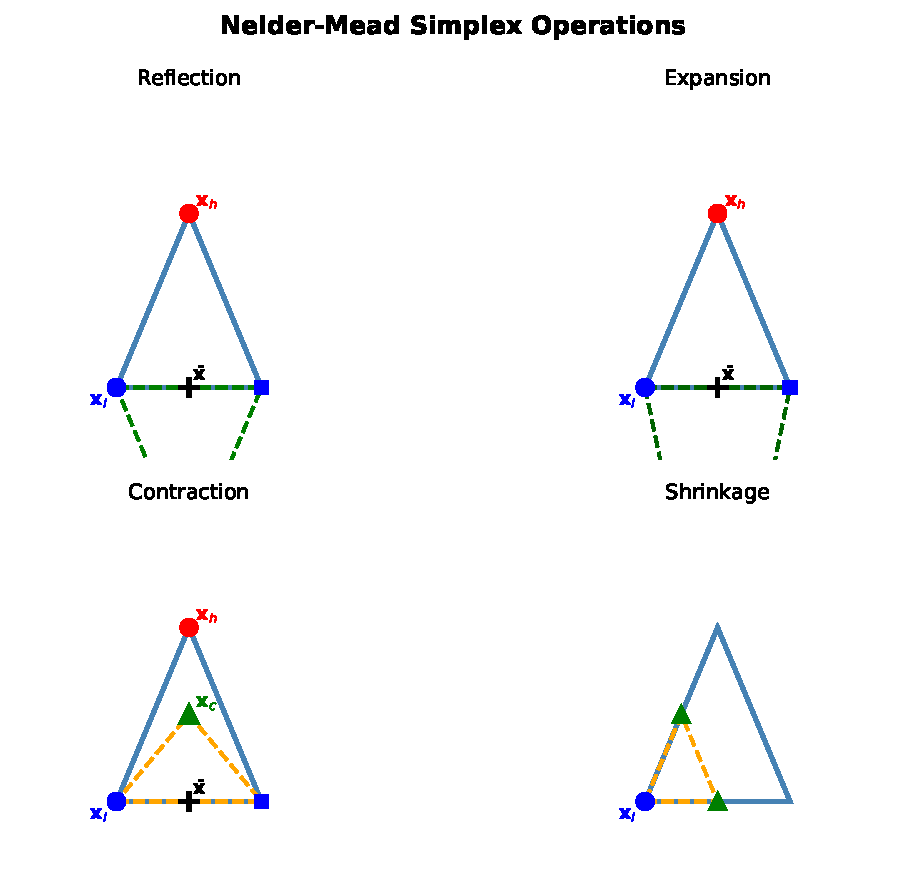
\includegraphics[width=\linewidth]{fig_nelder_mead_ops.pdf}\\
        {\scriptsize The four Nelder-Mead operations applied to a
        triangle in $\mathbb{R}^2$.  The worst vertex $\mathbf{x}_h$
        is moved relative to the centroid $\bar{\mathbf{x}}$ of the
        remaining edge.}
      \end{center}
  \end{columns}
\end{frame}

\begin{frame}[allowframebreaks]{7.5 Nelder-Mead --- Four Operations}
  Every iteration of Nelder-Mead chooses exactly one of four
  geometric operations to apply to the worst vertex.  The choice
  depends on how well the candidate new point compares to the
  existing vertices.

  \begin{columns}[T]
    \column{0.54\textwidth}
      \begin{block}{Operation 1: Reflection ($\alpha$, ``alpha'' $> 0$)}
        The most basic operation: reflect the worst vertex
        $\mathbf{x}_h$ over the centroid $\bar{\mathbf{x}}$:
        \[
          \mathbf{x}_r = \bar{\mathbf{x}} + \alpha(\bar{\mathbf{x}} - \mathbf{x}_h)
        \]
        This moves $\mathbf{x}_h$ to the \emph{opposite side} of the
        centroid.  Typically $\alpha = 1$, giving $\mathbf{x}_r =
        2\bar{\mathbf{x}} - \mathbf{x}_h$.

        The idea: if the minimum is in the direction away from the
        worst vertex, reflecting moves us toward it.
      \end{block}

      \begin{block}{Operation 2: Expansion ($\beta$, ``beta'' $> \max(1,\alpha)$)}
        If the reflected point $\mathbf{x}_r$ is the best point seen
        so far ($y_r < y_l$), try going even further in the same
        direction:
        \[
          \mathbf{x}_e = \bar{\mathbf{x}} + \beta(\mathbf{x}_r - \bar{\mathbf{x}})
        \]
        With $\beta = 2$, this extends the move to twice the
        reflected distance.  If $\mathbf{x}_e$ is better than
        $\mathbf{x}_r$, use it; otherwise use $\mathbf{x}_r$.
      \end{block}

      \begin{block}{Operation 3: Contraction ($\gamma$, ``gamma'' $\in (0,1)$)}
        If the reflected point is not an improvement, try a point
        between $\mathbf{x}_h$ and the centroid:
        \[
          \mathbf{x}_c = \bar{\mathbf{x}} + \gamma(\mathbf{x}_h - \bar{\mathbf{x}})
        \]
        With $\gamma = 0.5$, this puts the new point halfway between
        the centroid and the worst vertex.  This shrinks the simplex
        from the bad side.
      \end{block}
    \column{0.43\textwidth}
      \begin{block}{Operation 4: Shrinkage}
        If none of the above yields improvement, shrink the
        \emph{entire} simplex toward the best point $\mathbf{x}_l$:
        \[
          \mathbf{x}^{(i)} \leftarrow
          \frac{\mathbf{x}^{(i)} + \mathbf{x}_l}{2}, \quad i \ne l
        \]
        This moves every vertex (except the best) halfway toward the
        current best.  Shrinkage is expensive because it requires
        re-evaluating $f$ at $n$ new points.  It is used as a last
        resort when the simplex is poorly shaped.
      \end{block}

      \begin{block}{Convergence Criterion}
        The algorithm stops when the spread of function values across
        the simplex is small:
        \[
          \Delta = \text{std}\!\left(y^{(1)},\ldots,y^{(n+1)}\right) < \epsilon
        \]
        where $\text{std}$ (standard deviation, ``sigma'') measures
        how spread out the $n+1$ function values are.  A small
        $\Delta$ (delta) means all vertices have nearly the same
        function value, so the simplex has converged onto a flat region
        near the minimum.  A large $\Delta$ means the simplex spans a
        region where $f$ varies substantially, and the algorithm should
        keep working.
      \end{block}

      \begin{alertblock}{Key Insight on Parameters}
        The recommended parameter values are $\alpha=1$, $\beta=2$,
        $\gamma=0.5$.  The reflection parameter $\alpha$ controls the
        distance of the reflected point from the centroid.  Larger
        $\beta$ makes the expansion bolder.  Smaller $\gamma$ makes
        the contraction more conservative.  These defaults work well
        for most smooth functions in low dimensions.
      \end{alertblock}
  \end{columns}
\end{frame}

\begin{frame}{7.5 Nelder-Mead --- Decision Flowchart}
  \begin{center}
  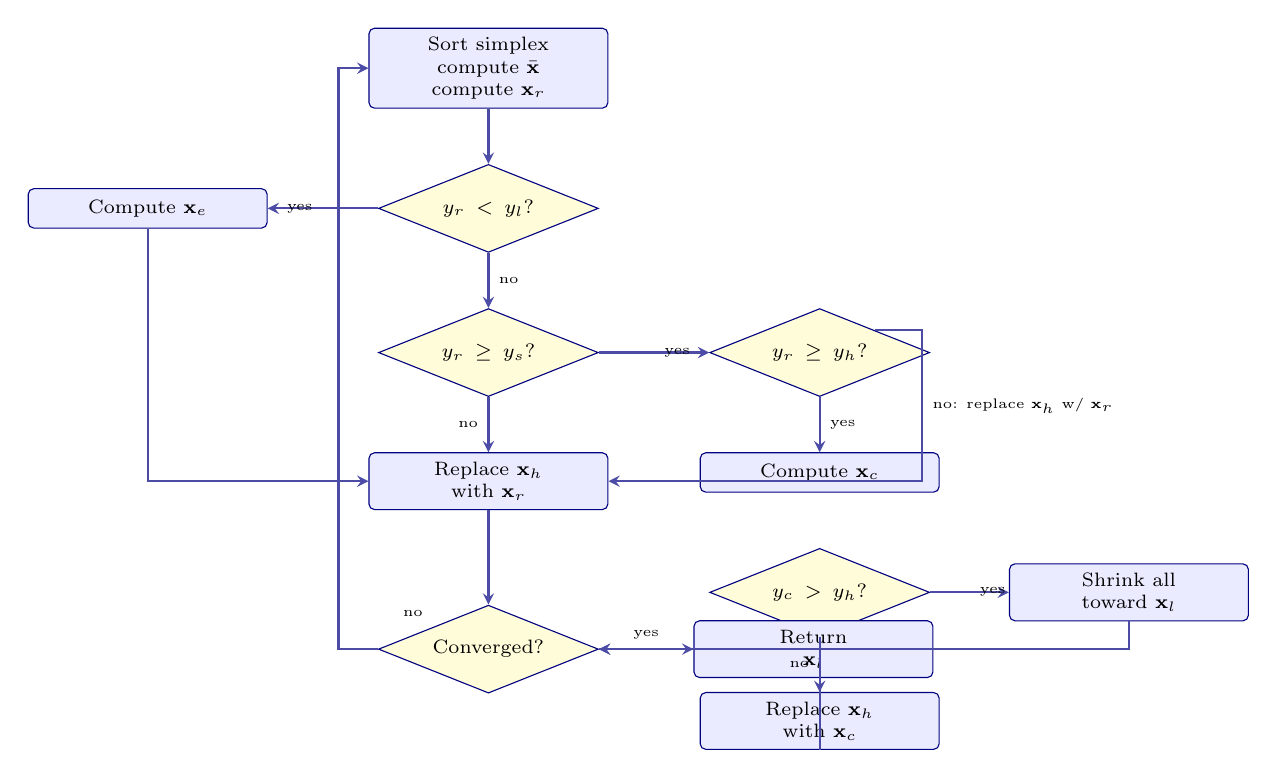
\begin{tikzpicture}[
      node distance=0.7cm and 0.8cm,
      box/.style={rectangle, draw=navy, rounded corners=2pt,
                  fill=blue!8, text width=2.8cm, align=center,
                  font=\scriptsize, minimum height=0.5cm},
      decision/.style={diamond, draw=navy, fill=yellow!15,
                       font=\scriptsize, aspect=2.5,
                       inner sep=1pt, text width=2.0cm, align=center},
      arr/.style={->, thick, >=stealth, draw=navy!70},
      ]
    \node[box] (init) {Sort simplex\\compute $\bar{\mathbf{x}}$\\compute $\mathbf{x}_r$};
    \node[decision, below=of init] (d1) {$y_r < y_l$?};
    \node[box, left=1.4cm of d1] (exp) {Compute $\mathbf{x}_e$};
    \node[decision, below=of d1] (d2) {$y_r \ge y_s$?};
    \node[decision, right=1.4cm of d2] (d3) {$y_r \ge y_h$?};
    \node[box, below=of d2] (repl_r2) {Replace $\mathbf{x}_h$\\with $\mathbf{x}_r$};
    \node[box, below=of d3] (contract) {Compute $\mathbf{x}_c$};
    \node[decision, below=of contract] (d4) {$y_c > y_h$?};
    \node[box, right=1.0cm of d4] (shrink) {Shrink all\\toward $\mathbf{x}_l$};
    \node[box, below=of d4] (repl_c) {Replace $\mathbf{x}_h$\\with $\mathbf{x}_c$};
    \node[decision, below=1.2cm of repl_r2] (conv) {Converged?};
    \node[box, right=1.2cm of conv] (ret) {Return\\$\mathbf{x}_l$};

    \draw[arr] (init) -- (d1);
    \draw[arr] (d1) -- node[left,font=\tiny]{yes} (exp);
    \draw[arr] (d1) -- node[right,font=\tiny]{no} (d2);
    \draw[arr] (d2) -- node[right,font=\tiny]{yes} (d3);
    \draw[arr] (d2) -- node[left,font=\tiny]{no} (repl_r2);
    \draw[arr] (d3) -- node[right,font=\tiny]{yes} (contract);
    \draw[arr] (d3.north east) -- ++(0.6,0) |- node[near start,right,font=\tiny]{no: replace $\mathbf{x}_h$ w/ $\mathbf{x}_r$} (repl_r2);
    \draw[arr] (d4) -- node[right,font=\tiny]{yes} (shrink);
    \draw[arr] (d4) -- node[left,font=\tiny]{no} (repl_c);
    \draw[arr] (exp.south) |- (repl_r2.west);
    \draw[arr] (repl_r2) -- (conv);
    \draw[arr] (repl_c.south) |- (conv.east);
    \draw[arr] (shrink.south) |- (conv.east);
    \draw[arr] (conv) -- node[above,font=\tiny]{yes} (ret);
    \draw[arr] (conv.west) -- ++(-0.5,0) |- (init.west);
    \node[font=\tiny,above left=0.01cm of conv] {no};
  \end{tikzpicture}
  \end{center}
\end{frame}

\begin{frame}[fragile]{7.5 Nelder-Mead --- Python Implementation}
\begin{lstlisting}[style=python, caption={Nelder-Mead simplex method (pure Python + SciPy)}]
import numpy as np
from scipy.optimize import minimize

def nelder_mead(f, simplex, eps=1e-6, alpha=1.0, beta=2.0, gamma=0.5):
    """
    Nelder-Mead simplex method.
    f       : callable R^n -> R
    simplex : list/array of (n+1) initial vertices, shape (n+1, n)
    alpha   : reflection coefficient  (> 0,   typically 1.0)
    beta    : expansion coefficient   (> 1,   typically 2.0)
    gamma   : contraction coefficient (in (0,1), typically 0.5)
    """
    S = [np.array(s, dtype=float) for s in simplex]
    while True:
        y = np.array([f(s) for s in S])
        p = np.argsort(y)
        S = [S[i] for i in p]; y = y[p]
        if np.std(y) < eps:      # convergence check
            break
        xl, yl = S[0], y[0]     # best vertex
        xh, yh = S[-1], y[-1]   # worst vertex
        xs, ys = S[-2], y[-2]   # second-worst vertex
        xm = np.mean(S[:-1], axis=0)         # centroid (excluding worst)
        xr = xm + alpha * (xm - xh)          # reflection
        yr = f(xr)
        if yr < yl:                           # reflected point is new best
            xe = xm + beta * (xr - xm)       # try expansion
            S[-1] = xe if f(xe) < yr else xr
        elif yr >= ys:                        # reflection not good enough
            if yr < yh: xh, yh = xr, yr; S[-1] = xr
            xc = xm + gamma * (xh - xm)      # contraction
            if f(xc) > yh:                   # contraction failed: shrink
                for i in range(1, len(S)):
                    S[i] = (S[i] + xl) / 2
            else:
                S[-1] = xc
        else:
            S[-1] = xr                       # accept reflected point
    return S[0]

# SciPy's built-in Nelder-Mead (recommended for production use):
result = minimize(lambda v: (1-v[0])**2 + 100*(v[1]-v[0]**2)**2,
                  [-1.2, 1.0], method='Nelder-Mead')
print(result.x)  # -> [1. 1.]
\end{lstlisting}
\end{frame}

\begin{frame}[allowframebreaks]{7.5 Nelder-Mead --- Iterations Visualised}
  \begin{center}
    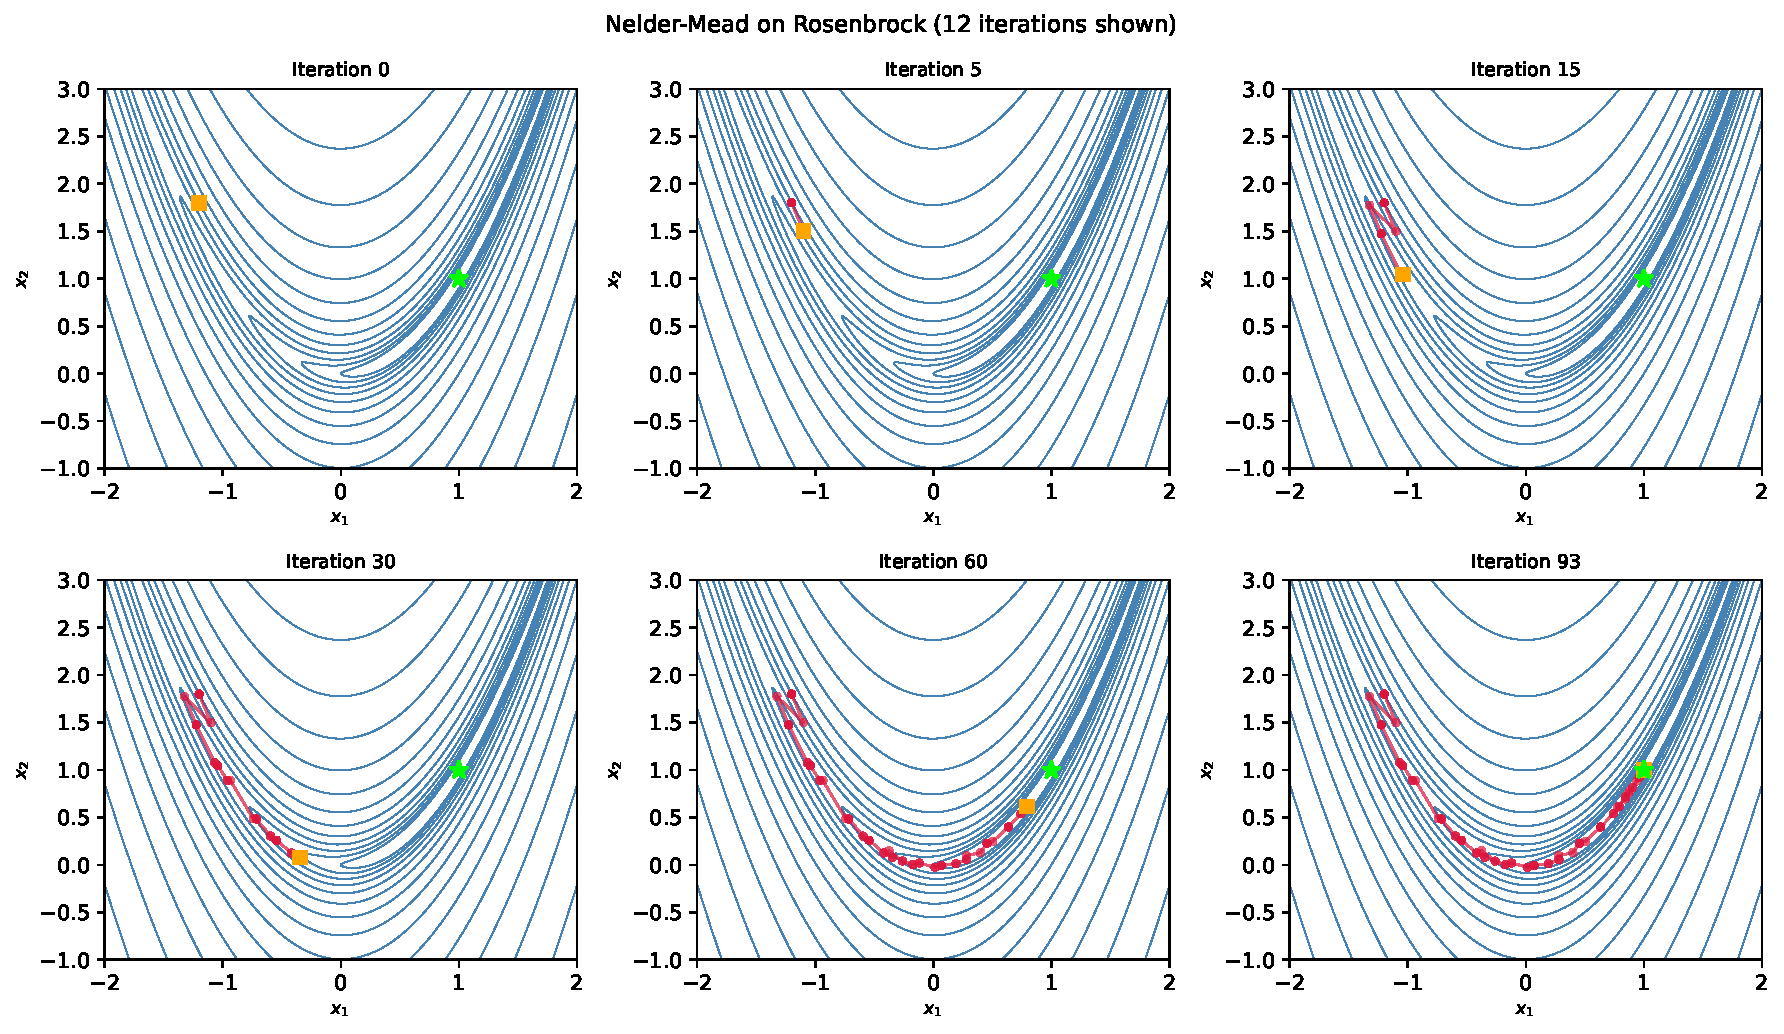
\includegraphics[width=0.85\linewidth]{fig_nelder_mead_iters.pdf}
  \end{center}
  \vspace{-2mm}
  {\small The figure shows Nelder-Mead applied to the Rosenbrock
  function $f(x_1,x_2) = (1-x_1)^2 + 100(x_2-x_1^2)^2$, which has
  a narrow curved valley with its minimum at $(1,\,1)$.

  In the \textbf{early iterations}, the simplex is large and uses
  mostly reflection and expansion to move quickly across the landscape.
  As the simplex enters the narrow valley, contractions become necessary
  to track the curve of the valley.  In the \textbf{late iterations},
  the simplex becomes very small and performs many shrinkages to tighten
  around the minimum.  The total number of function evaluations is
  moderate (typically a few hundred for this 2D problem), which is why
  Nelder-Mead is popular for low-dimensional problems in practice.}

  \begin{alertblock}{Limitation: No Convergence Guarantee}
    Unlike GPS, Nelder-Mead has \emph{no formal convergence guarantee}
    for general non-convex functions.  The simplex can collapse onto a
    non-stationary point, especially in high dimensions ($n > 5$).
    Despite this limitation, Nelder-Mead works well empirically for
    smooth functions in low dimensions and is the standard
    derivative-free optimiser in many scientific computing packages.
  \end{alertblock}
\end{frame}

%======================================================================
\section{Divided Rectangles (DIRECT)}
%======================================================================

\begin{frame}[allowframebreaks]{7.6 DIRECT --- Overview and Lipschitz Condition}
  The methods we have studied so far --- cyclic search, Powell,
  Hooke-Jeeves, GPS, Nelder-Mead --- are all \emph{local} methods.
  They converge to a minimum near the starting point but may miss
  the global minimum.  \textbf{DIRECT} (DIvided RECTangles, Jones et al.
  1993) is designed for \emph{global} optimisation: it provides
  a principled way to search the entire bounded domain
  $[\mathbf{a},\mathbf{b}]$ and is guaranteed to converge to the
  global minimum given enough iterations.

  \begin{columns}[T]
    \column{0.54\textwidth}
      \begin{block}{The Setting: Bounded, Lipschitz-Continuous $f$}
        DIRECT applies to problems of the form:
        \[
          \min_{\mathbf{x} \in [\mathbf{a},\,\mathbf{b}]} f(\mathbf{x})
        \]
        where $\mathbf{a},\mathbf{b} \in \mathbb{R}^n$ are known lower
        and upper bounds on each variable, and $f$ is
        \emph{Lipschitz-continuous} --- meaning it cannot change too
        rapidly.
      \end{block}

      \begin{block}{The Lipschitz Condition}
        The function $f$ satisfies a Lipschitz condition with constant
        $\ell$ (ell) if, for every pair of points $\mathbf{x}$ and
        $\mathbf{y}$ in the domain:
        \[
          \bigl|f(\mathbf{x}) - f(\mathbf{y})\bigr|
          \le \ell\,\|\mathbf{x} - \mathbf{y}\|
        \]
        Here $|\cdot|$ denotes the absolute value, and
        $\|\cdot\|$ (the Euclidean norm) measures the distance between
        the two points.  The constant $\ell$ (ell, also called the
        Lipschitz constant) is the maximum rate at which $f$ can change.
      \end{block}

      \begin{alertblock}{How to Read the Lipschitz Condition}
        This condition says that if two points are close together
        (small $\|\mathbf{x}-\mathbf{y}\|$), their function values
        cannot differ by much.  Equivalently, the function has bounded
        slope --- it cannot jump.  This is a mild requirement satisfied
        by virtually all continuously differentiable functions.  The
        Lipschitz constant $\ell$ is the ``maximum speed'' at which $f$
        can increase or decrease.
      \end{alertblock}
    \column{0.43\textwidth}
      \begin{block}{Lower Bound from the Lipschitz Condition}
        Given that $f$ is evaluated at a center point $\mathbf{c}$,
        and that any point $\mathbf{x}$ in an interval around
        $\mathbf{c}$ is at most distance $r$ (the radius) from $\mathbf{c}$,
        the Lipschitz condition provides a lower bound:
        \[
          f(\mathbf{x}) \ge f(\mathbf{c}) - \ell\,r
          \quad \text{for all } \mathbf{x} \text{ in the interval}
        \]
        This says: the smallest $f$ can be anywhere in the interval is
        $f(\mathbf{c}) - \ell r$.  We do not know $\ell$, but DIRECT
        avoids this by considering \emph{all} possible values of $\ell
        \ge 0$.
      \end{block}

      \begin{center}
        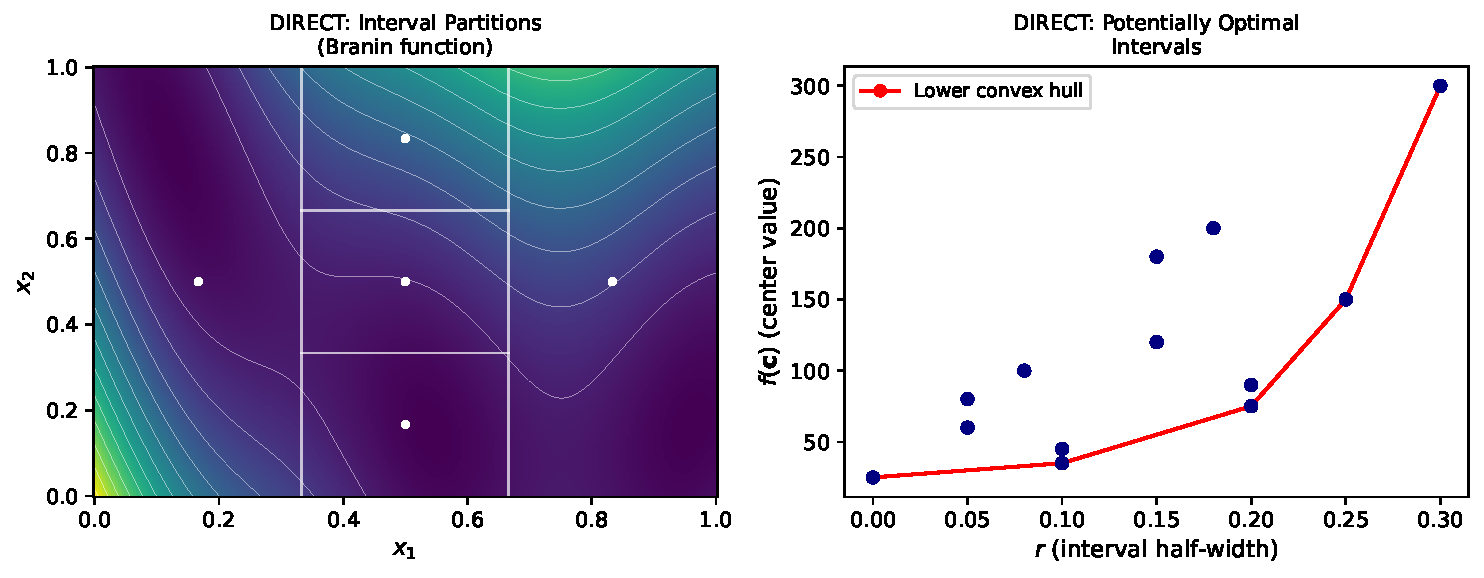
\includegraphics[width=\linewidth]{fig_direct_partitioning.pdf}\\
        {\scriptsize Left: DIRECT interval partitions superimposed on
        the Branin function contour plot.  Right: scatter of
        $(r, f(\mathbf{c}))$ pairs for each interval, with the lower
        convex hull (red) identifying potentially optimal intervals.}
      \end{center}
  \end{columns}
\end{frame}

\begin{frame}[allowframebreaks]{7.6 DIRECT --- Potentially Optimal Intervals}
  The key challenge in global optimisation is deciding \emph{which}
  region to explore next.  Exploring every region equally is
  wasteful; ignoring a region risks missing the global minimum.
  DIRECT uses the concept of \emph{potentially optimal intervals}
  to balance exploration (sampling new regions) with exploitation
  (refining promising regions).

  \begin{columns}[T]
    \column{0.54\textwidth}
      \begin{block}{Definition: Potentially Optimal Interval}
        An interval $I$ with center $\mathbf{c}$ and radius $r$
        (half-diagonal) is \textbf{potentially optimal} if there
        exists some Lipschitz constant $\ell \ge 0$ such that both
        conditions hold:
        \begin{enumerate}\setlength\itemsep{3pt}
          \item $f(\mathbf{c}) - \ell\,r \le f(\mathbf{c}') - \ell\,r'$
                for every other interval $I'$ with center $\mathbf{c}'$
                and radius $r'$.
                (This interval's lower bound is as good as any other's.)
          \item $f(\mathbf{c}) - \ell\,r \le f_{\min} - \epsilon_{\text{DIRECT}}
                |f_{\min}|$
                where $f_{\min}$ is the best value found so far.
                (The potential improvement is worth exploring.)
        \end{enumerate}
      \end{block}

      \begin{block}{Geometric Interpretation}
        Geometrically, the potentially optimal intervals correspond to
        points on the \textbf{lower-right convex hull} of the scatter
        plot of $(r, f(\mathbf{c}))$ pairs for all current intervals.
        The lower-right convex hull consists of the points that are not
        dominated --- no other point is simultaneously at a smaller
        radius and smaller function value.  Each point on this hull
        is potentially optimal for some value of $\ell$.
      \end{block}

      \begin{alertblock}{Key Insight}
        The potentially optimal condition elegantly sidesteps the need
        to know $\ell$ in advance.  By selecting all intervals that
        are optimal \emph{for some} $\ell \ge 0$, DIRECT guarantees
        that no promising region is overlooked.  As iterations proceed,
        the convex hull becomes more refined and the algorithm focuses
        on smaller and smaller regions near the global minimum.
      \end{alertblock}

    \column{0.43\textwidth}
      \begin{block}{Splitting Rule}
        When an interval is selected as potentially optimal, it is
        split along its \emph{longest} dimension into
        \textbf{three equal parts}.  The two new center points are
        evaluated, and the three sub-intervals replace the original:
        \[
          r_{\text{new}} = \frac{r_{\text{old}}}{3}
        \]
        Splitting along the longest dimension first ensures that all
        dimensions are eventually refined uniformly.  The sub-interval
        with the smallest function value at its center is split first,
        so promising sub-regions get priority.
      \end{block}

      \begin{center}
        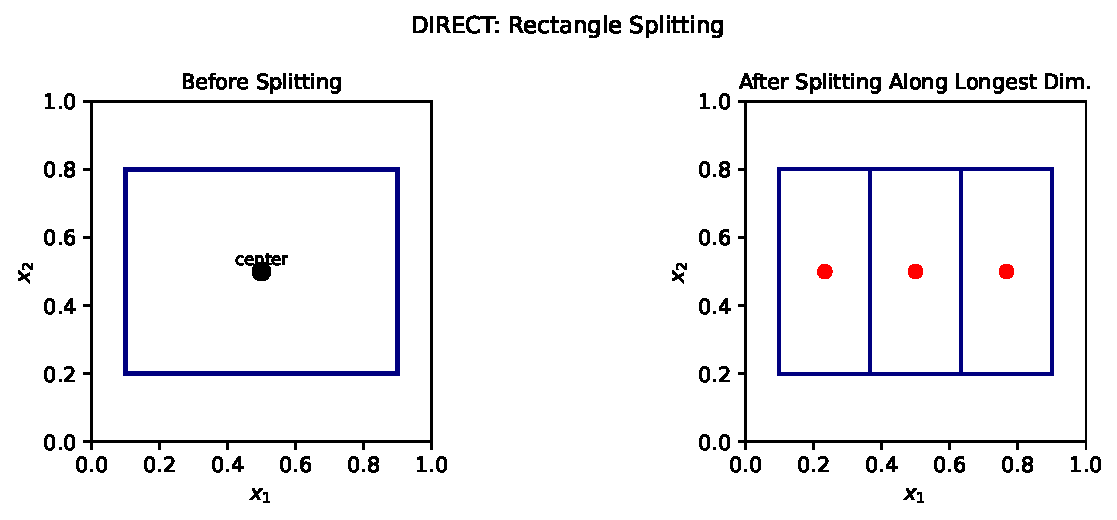
\includegraphics[width=\linewidth]{fig_direct_splitting.pdf}\\
        {\scriptsize DIRECT splits each selected interval into three
        equal thirds along the longest dimension.  After $k$ splits on
        dimension $i$, the width in that dimension shrinks by factor
        $3^{-k}$.}
      \end{center}

      \begin{block}{Radius After Multiple Splits}
        In $n$ dimensions, after $d_i$ splits along dimension $i$,
        the half-diagonal radius of the sub-interval is:
        \[
          r = \sqrt{\sum_{i=1}^n \left(\frac{1}{2}\cdot\frac{1}{3^{d_i}}\right)^{\!2}}
        \]
        where $d_i$ (``$d$-sub-$i$'') counts how many times dimension
        $i$ has been split, and the sum $\sum_{i=1}^n$ (Sigma from
        $i=1$ to $n$) adds the squared half-widths over all $n$
        dimensions.  As $d_i$ grows, $3^{-d_i}$ shrinks rapidly,
        so deeply-split intervals have very small radius.
      \end{block}
  \end{columns}
\end{frame}

\begin{frame}[allowframebreaks]{7.6 DIRECT --- Algorithm}
  \begin{columns}[T]
    \column{0.55\textwidth}
      \begin{alertblock}{Algorithm 7.8 --- DIRECT}
        \textbf{Inputs:} $f$, lower bounds $\mathbf{a}$, upper bounds
        $\mathbf{b}$, maximum iterations $k_{\max}$, minimum radius
        $r_{\min}$.

        \begin{enumerate}\setlength\itemsep{1pt}
          \item \textbf{Normalise} the domain: define a helper function
                $g(\mathbf{x}') = f(\mathbf{x}' \cdot (\mathbf{b}-\mathbf{a}) + \mathbf{a})$
                that maps the unit hypercube $[0,1]^n$ back to
                $[\mathbf{a},\mathbf{b}]$.
          \item Initialise a single interval: center
                $\mathbf{c} = [0.5,\ldots,0.5]^\top$,
                radius $r = \sqrt{n}\cdot 0.5$,
                zero splits in all dimensions.
          \item Evaluate $g(\mathbf{c})$.
          \item \textbf{for} $k = 1,\ldots,k_{\max}$:
          \item \quad Identify all \emph{potentially optimal} intervals
                from the lower convex hull: call this set
                $\mathcal{S}_{\text{split}}$.
          \item \quad Remove those intervals from the collection $\mathcal{S}$.
          \item \quad For each interval in $\mathcal{S}_{\text{split}}$:
                split it into three, evaluate the two new centers,
                add all three sub-intervals back to $\mathcal{S}$.
          \item \quad Update the best-known point $\mathbf{c}_{\text{best}}$.
          \item \textbf{return} $\mathbf{c}_{\text{best}} \cdot
                (\mathbf{b}-\mathbf{a}) + \mathbf{a}$
                (map back to original coordinates).
        \end{enumerate}
      \end{alertblock}
    \column{0.42\textwidth}
      \begin{block}{The DirectRectangle Data Structure}
        Each interval is stored as a record with four fields:
        \begin{itemize}\setlength\itemsep{2pt}
          \item $\mathbf{c}$: the center point in the normalised unit
                hypercube $[0,1]^n$
          \item $y = g(\mathbf{c})$: the function value at the center
          \item $\mathbf{d} \in \mathbb{Z}^n_{\ge 0}$ (d, integer vector):
                the number of splits per dimension so far
          \item $r$: the half-diagonal radius (used for convex hull
                selection)
        \end{itemize}
      \end{block}

      \begin{block}{Implementation Note}
        An efficient implementation groups intervals by their radius
        value $r$ and, within each group, sorts by $f(\mathbf{c})$.
        This allows finding the lower convex hull in $O(K \log K)$
        time where $K$ is the number of distinct radii.  A min-heap
        (priority queue) per distinct radius supports $O(\log N)$
        insertion and retrieval.
      \end{block}

      \begin{block}{Global Convergence}
        DIRECT is guaranteed to find the global minimum as
        $k \to \infty$ (i.e., as the number of iterations grows without
        bound), because every region of the domain will eventually
        be split to arbitrary fineness.  In practice, the algorithm
        focuses on the most promising regions first, giving good
        approximate results after relatively few iterations.
      \end{block}
  \end{columns}
\end{frame}

\begin{frame}[fragile]{7.6 DIRECT --- Python Implementation}
\begin{lstlisting}[style=python, caption={DIRECT algorithm in Python}]
import numpy as np
from dataclasses import dataclass, field
from typing import List

@dataclass
class Rect:
    c: np.ndarray        # center in unit hypercube [0,1]^n
    y: float             # f(c): function value at center
    d: np.ndarray        # number of splits per dimension (integer)
    r: float             # half-diagonal radius

def direct(f, a, b, k_max=20, r_min=1e-4):
    """DIRECT algorithm for global optimisation over [a, b]."""
    a, b = np.asarray(a, float), np.asarray(b, float)
    n = len(a)
    # Map unit hypercube back to [a, b] for evaluating f
    g = lambda xp: f(xp * (b - a) + a)
    c = np.full(n, 0.5)
    rects = [Rect(c.copy(), g(c), np.zeros(n, int),
                  np.sqrt(n) * 0.5)]
    c_best = c.copy()
    for _ in range(k_max):
        # Find potentially optimal intervals (lower convex hull)
        to_split = _potentially_optimal(rects, r_min)
        new_rects = []
        for rect in to_split:
            rects.remove(rect)
            new_rects.extend(_split_rect(rect, g))
        rects.extend(new_rects)
        c_best = min(rects, key=lambda r: r.y).c
    return c_best * (b - a) + a

def _split_rect(rect, g):
    """Split along the least-split (longest) dimension, trisect."""
    d = rect.d.copy(); c = rect.c.copy()
    j = np.argmin(d)           # split the least-divided axis first
    delta = 3.0**(-d[j] - 1)  # one-third of current width in dim j
    subs = []
    for sign in (+1, -1):
        cn = c.copy(); cn[j] += sign * delta
        dn = d.copy(); dn[j] += 1
        rn = np.sqrt(np.sum((0.5 / 3**dn)**2))  # new radius
        subs.append(Rect(cn, g(cn), dn, rn))
    rect.d[j] += 1
    rect.r = np.sqrt(np.sum((0.5 / 3**rect.d)**2))
    return [rect] + subs
\end{lstlisting}
\end{frame}

\begin{frame}[allowframebreaks]{7.6 DIRECT --- Worked Example}
  \begin{columns}[T]
    \column{0.55\textwidth}
      \begin{exampleblock}{Example 7.1 --- Flower Function on $[-1,3]\times[-2,1]$}
        We want to minimise the \emph{flower function} over the
        rectangle $x_1 \in [-1,3]$, $x_2 \in [-2,1]$.

        \textbf{Normalisation.}  DIRECT first maps the domain to the
        unit square $[0,1]^2$ via:
        $x_1 = 4x_1' - 1$, $x_2 = 3x_2' - 2$.

        \textbf{Iteration 0.}  Sample at the center of the unit square,
        $[0.5,\,0.5]^\top$, which maps to $[1,\,-0.5]^\top$ in
        original coordinates.  Evaluate $g([0.5,0.5]) = 0.158$.

        \textbf{First Split.}  The single initial interval is trivially
        potentially optimal and is split along dimension 1 (the $x_1'$
        axis).  This creates five intervals (the original center plus
        two new centers for each split):
        \begin{center}
        \small
        \begin{tabular}{@{}ccccc@{}}
          \toprule
          Int. & Center & Width & $r$ & $f(\mathbf{c})$ \\
          \midrule
          1 & $[1/6,\;3/6]$ & $[1/3,1]$ & 0.527 & 0.500 \\
          2 & $[5/6,\;3/6]$ & $[1/3,1]$ & 0.527 & 1.231 \\
          3 & $[3/6,\;3/6]$ & $[1/3,1]$ & 0.236 & 0.158 \\
          4 & $[3/6,\;1/6]$ & $[1/3,1/3]$ & 0.236 & 2.029 \\
          5 & $[3/6,\;5/6]$ & $[1/3,1/3]$ & 0.236 & 1.861 \\
          \bottomrule
        \end{tabular}
        \end{center}
        Next: intervals 1 and 3 lie on the lower convex hull of the
        $(r, f(\mathbf{c}))$ scatter and will be split next.
      \end{exampleblock}
    \column{0.42\textwidth}
      \begin{center}
        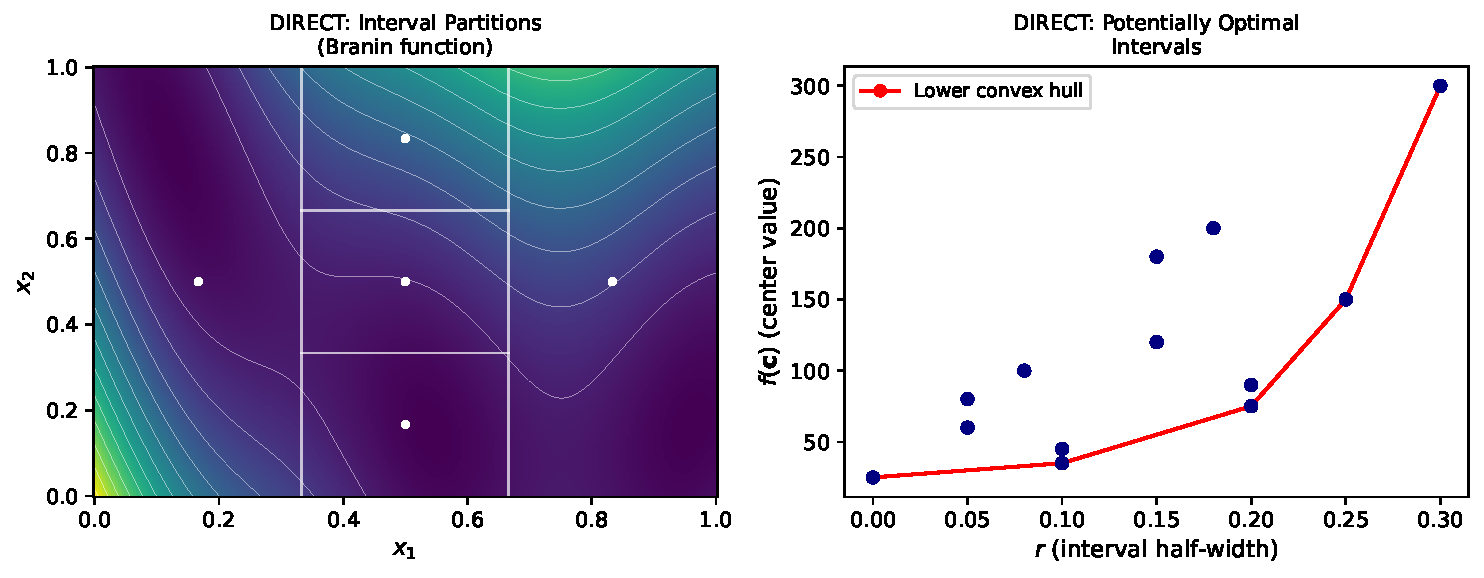
\includegraphics[width=\linewidth]{fig_direct_partitioning.pdf}\\
        {\scriptsize After several DIRECT iterations on the Branin
        function.  Left: spatial partitions show finer resolution near
        the two minima.  Right: the $(r, f(\mathbf{c}))$ scatter with
        the lower convex hull in red, identifying the intervals to be
        split next.}
      \end{center}

      \begin{block}{Reading the Table}
        Each row corresponds to one interval (a rectangle in the
        normalised domain).  The column ``Width'' gives the side lengths
        of the rectangle; ``$r$'' is the half-diagonal radius
        (a single number summarising the interval's size); and
        ``$f(\mathbf{c})$'' is the function value at the center.
        A small $r$ with a small $f(\mathbf{c})$ means a promising
        fine-grained region.  A large $r$ with a moderate $f(\mathbf{c})$
        may still be selected if it could contain the global minimum
        under some Lipschitz constant $\ell$.
      \end{block}
  \end{columns}
\end{frame}

%======================================================================
\section{Summary \& Exercises}
%======================================================================

\begin{frame}[allowframebreaks]{7.7 Summary}
  \begin{block}{The Role of Direct Methods}
    Direct methods occupy an important niche in optimisation:
    they require only the ability to evaluate $f(\mathbf{x})$, making
    them applicable to simulation-based, experimental, or legacy
    black-box problems where derivatives are simply unavailable.
    The trade-off is that they typically require more function
    evaluations than gradient-based methods, and most of them offer
    only local convergence guarantees.
  \end{block}

  \begin{columns}[T]
    \column{0.48\textwidth}
      \begin{block}{Cyclic Coordinate Search}
        Optimises one variable at a time via line search, cycling
        through all $n$ coordinate directions repeatedly.  It is the
        simplest direct method and works well for \emph{separable}
        functions where the variables affect $f$ independently.  It is
        slow on diagonally-oriented valleys because it cannot move
        diagonally.  An acceleration step (adding the net-displacement
        direction after each cycle) can significantly improve speed.
      \end{block}
      \begin{block}{Powell's Method}
        Builds up a set of \emph{conjugate} search directions that are
        better aligned with the geometry of $f$.  Achieves faster
        convergence than cyclic search, and for quadratic objectives
        converges in exactly $n$ steps.  The direction set may
        degrade (lose conjugacy) on highly non-quadratic functions,
        requiring periodic reinitialisation.
      \end{block}
      \begin{block}{Hooke-Jeeves Method}
        Combines an exploratory search (probing $\pm\alpha\mathbf{e}^{(i)}$
        in each coordinate direction) with a pattern move (extrapolating
        along the direction of improvement).  Uses $2n$ function
        evaluations per iteration.  Provably convergent for continuous
        functions.  An accessible and reliable general-purpose method.
      \end{block}
    \column{0.48\textwidth}
      \begin{block}{Generalized Pattern Search}
        Generalises Hooke-Jeeves to allow any positive spanning set
        $\mathcal{D}$ of directions, not just the coordinate axes.
        All evaluated points lie on a scaled lattice.  Under mild
        continuity conditions, convergence to a stationary point is
        guaranteed --- stronger than Hooke-Jeeves.  Particularly
        useful when coordinate directions are inefficient or
        infeasible.
      \end{block}
      \begin{block}{Nelder-Mead Simplex}
        Maintains a simplex of $n+1$ vertices and deforms it each
        iteration via reflection, expansion, contraction, or
        shrinkage.  Requires only 1 to $n+1$ function evaluations per
        iteration.  Widely used in practice (the default in SciPy for
        derivative-free optimisation) and works well empirically for
        smooth low-dimensional problems.  Has no formal convergence
        guarantee for general non-convex functions.
      \end{block}
      \begin{block}{DIRECT}
        A global optimisation method for Lipschitz-continuous functions
        on a bounded domain.  Recursively partitions the domain into
        intervals and uses the lower convex hull of the $(r, f(\mathbf{c}))$
        scatter to identify \emph{potentially optimal} intervals for
        splitting.  Avoids the need to know the Lipschitz constant $\ell$.
        Guaranteed to find the global minimum as $k \to \infty$.
        Memory grows as $O(3^k)$ in the worst case.
      \end{block}
  \end{columns}

  \framebreak

  \begin{center}
    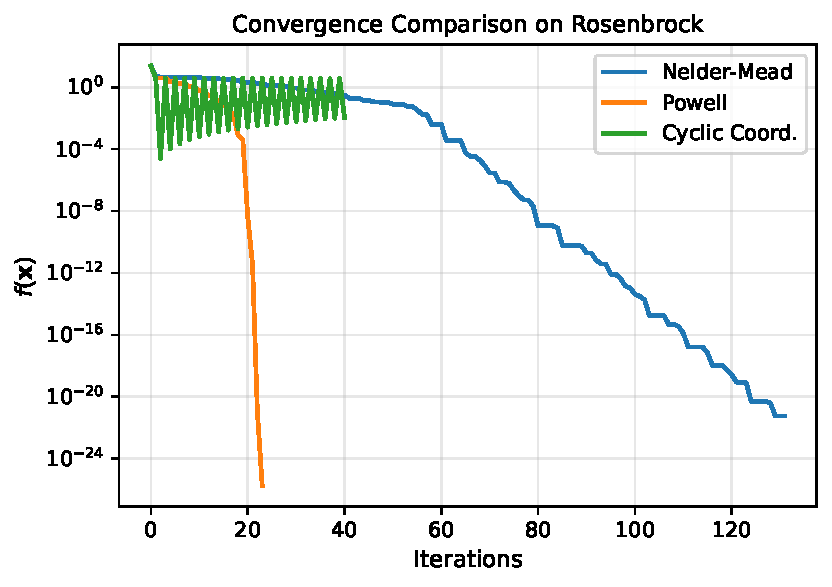
\includegraphics[width=0.6\linewidth]{fig_convergence_comparison.pdf}\\
    {\small Convergence comparison on the Rosenbrock function.
    Nelder-Mead and Powell's method converge significantly faster
    (in terms of function evaluations) than cyclic coordinate search.
    This illustrates the benefit of adaptively building better search
    directions.}
  \end{center}

  \begin{block}{Method Comparison Table}
    \centering
    \small
    \begin{tabular}{lcccc}
      \toprule
      Method & Global? & Evals/iter & Memory & Best for \\
      \midrule
      Cyclic coord. & No & $n$ & $O(n)$ & Separable $f$ \\
      Powell        & No & $n \cdot (\text{line search})$ & $O(n^2)$ & Smooth $f$ \\
      Hooke-Jeeves  & No & $2n$ & $O(n)$ & General $f$ \\
      GPS           & No & $|\mathcal{D}|$ & $O(n|\mathcal{D}|)$ & Constrained lattice \\
      Nelder-Mead   & No & $1$--$n+1$ & $O(n^2)$ & Low-dim, smooth $f$ \\
      DIRECT        & Yes & $2n$ per split & $O(3^k)$ & Bounded, Lipschitz $f$ \\
      \bottomrule
    \end{tabular}
  \end{block}

  \begin{alertblock}{Key Takeaway}
    There is no single best direct method.  The choice depends on
    the problem: for smooth, low-dimensional problems Nelder-Mead is
    a reliable first choice; for problems with structure (separability
    or known geometry) cyclic search or GPS may be more efficient;
    for global search over a bounded domain, DIRECT is the principled
    choice.  All direct methods share the fundamental trade-off that
    more function evaluations yield better accuracy, but with
    diminishing returns as the algorithm hones in on the minimum.
  \end{alertblock}
\end{frame}

\begin{frame}[allowframebreaks]{7.8 Exercises}
  The following exercises are designed to deepen understanding of
  the methods in this chapter.  Some require pencil-and-paper analysis;
  others suggest computational experiments.

  \begin{exampleblock}{Exercise 7.1 --- Hooke-Jeeves Failure Case}
    Design an objective function $f$ and a starting point
    $\mathbf{x}^{(0)}$ such that the Hooke-Jeeves method fails to
    reduce $f$ at the very first step (i.e., the exploratory phase
    finds no improvement in any coordinate direction with step size
    $\alpha$).  What does this imply about the algorithm's behaviour?
    Does the algorithm eventually recover and converge, or does it
    stall permanently?

    \medskip
    \textit{Hint: Consider a function whose minimum lies in a region
    that is never reached by coordinate-aligned steps of size $\alpha$
    from the starting point.  Also consider what happens to $\alpha$
    as the algorithm progresses.}
  \end{exampleblock}

  \begin{exampleblock}{Exercise 7.2 --- Why Cyclic Search Improves Each Cycle}
    Explain in your own words why cyclic coordinate search is guaranteed
    to find an improvement (or confirm a minimum) after each full cycle
    through all $n$ coordinates, provided the current point is not a
    local minimum.  Then identify the condition on $f$ that breaks this
    guarantee, giving a specific example.

    \medskip
    \textit{Hint: Think about what ``not a local minimum'' means for a
    function that is differentiable.  Then consider a function with
    a flat plateau or a non-differentiable kink.}
  \end{exampleblock}

  \begin{exampleblock}{Exercise 7.3 --- GPS Beats Cyclic Search}
    Give a concrete two-dimensional objective function $f(x_1, x_2)$
    for which cyclic coordinate search with the standard $\pm\mathbf{e}^{(i)}$
    directions will stall at a non-optimal point (i.e., every step
    in a coordinate direction increases $f$, even though a diagonal
    step would decrease it).  Then describe how GPS with a richer
    direction set $\mathcal{D}$ that includes diagonal directions would
    succeed in finding a better point from the same starting location.
  \end{exampleblock}

  \framebreak

  \begin{exampleblock}{Exercise 7.4 --- DIRECT vs.\ Nelder-Mead: Theoretical Comparison}
    Explain the fundamental structural difference between the DIRECT
    algorithm and the Nelder-Mead simplex method.  Your answer should
    address: (a) what each method maintains in memory, (b) how each
    method decides where to evaluate $f$ next, and (c) what
    convergence guarantee (if any) each method provides.

    \medskip
    \textit{Solution sketch:}
    DIRECT maintains a collection of non-overlapping rectangles that
    tile the entire search domain, whereas Nelder-Mead maintains a
    single simplex of $n+1$ points that moves freely through the space.
    DIRECT's selection of intervals via the lower convex hull gives a
    global coverage guarantee; Nelder-Mead has no such guarantee.
    For a 2D problem with $n=2$, each split of DIRECT evaluates
    $2n = 4$ new points; after $k=5$ iterations the total number of
    rectangles grows at most as $O(3^5) = 243$, though typically far
    fewer are split each iteration.
  \end{exampleblock}

  \begin{exampleblock}{Exercise 7.5 --- Computational Experiment (Multimodal)}
    Find the global minimum of the multimodal function:
    \[
      f(x_1, x_2) = \sin\!\bigl(\tfrac{1}{2}x_1^2 - \tfrac{1}{4}x_2^2 + 3\bigr)
      \cos(2x_1 + 1 - e^{x_2})
    \]
    over $x_1, x_2 \in [-2, 2]$ using the two approaches below.
    Compare the solutions found and discuss which method is more
    reliable for this multimodal (many-local-minima) function.

    \medskip
    \textbf{(a) Nelder-Mead:} Run the algorithm from three different
    starting simplices (e.g., centred at $[-1.5,-1.5]$, $[0,0]$, and
    $[1.5,1.5]$).  Use:
    \texttt{scipy.optimize.minimize(f, x0, method='Nelder-Mead')}.

    \textbf{(b) DIRECT:} Run the global search directly using:
    \texttt{scipy.optimize.direct(f, bounds=[(-2,2),(-2,2)])}.

    \medskip
    \textit{Hint: Nelder-Mead is sensitive to the starting simplex
    on this function and may find different local minima from different
    starting points.  DIRECT should reliably find the global minimum
    regardless of initialisation.}
  \end{exampleblock}
\end{frame}

%──────────────────────────────────────────────────────────────────────
\begin{frame}{References}
  \begin{thebibliography}{9}
    \bibitem{kw2026}
      M.~J. Kochenderfer and T.~A. Wheeler,
      \emph{Algorithms for Optimization}, 2nd ed.,
      MIT Press, 2026.
    \bibitem{hookejeeves}
      R.~Hooke and T.~A. Jeeves,
      ``Direct Search Solution of Numerical and Statistical
      Problems,''
      \emph{Journal of the ACM}, vol.~8, no.~2, pp.~212--229, 1961.
    \bibitem{nelder1965}
      J.~A. Nelder and R.~Mead,
      ``A Simplex Method for Function Minimization,''
      \emph{The Computer Journal}, vol.~7, no.~4,
      pp.~308--313, 1965.
    \bibitem{jones1993}
      D.~R. Jones, C.~D. Perttunen, and B.~E. Stuckman,
      ``Lipschitzian Optimization Without the Lipschitz Constant,''
      \emph{Journal of Optimization Theory and Applications},
      vol.~79, no.~1, pp.~157--181, 1993.
    \bibitem{regis2016}
      R.~G. Regis,
      ``On the Properties of Positive Spanning Sets and Positive
      Bases,''
      \emph{Optimization and Engineering}, vol.~17, no.~1,
      pp.~229--262, 2016.
  \end{thebibliography}
\end{frame}

%──────────────────────────────────────────────────────────────────────
\end{document}
